\documentclass[sigconf, nonacm]{vldb/acmart}
\usepackage{caption}
\usepackage{subcaption}
\usepackage[linesnumbered,ruled,vlined]{algorithm2e}
\usepackage{setspace}
% \usepackage{algorithm}
% \usepackage{algorithmic}
\usepackage{enumitem}
% \usepackage{ulem}
% \usepackage{float}
\usepackage{stfloats}
\usepackage{graphicx}
\usepackage{pifont}
\usepackage{url}
\usepackage{balance}
\usepackage[normalem]{ulem}
\usepackage[a-2b,mathxmp]{pdfx}
\usepackage{amsmath}
\usepackage{multicol}
\usepackage{multirow}
\usepackage{booktabs}
\usepackage{makecell}
\usepackage{utfsym}
\usepackage{xspace}
\usepackage{framed}

% custom style
\usepackage{commons/code}
\usepackage{commons/colors}

\usepackage{amsthm}
\newtheorem{definition}{Definition}
\newtheorem{example}{Example}
\newtheorem{corollary}{Corollary}

% balance last page
\usepackage{balance}

% whether page numbers should be shown or not, use 'plain' for review versions, 'empty' for camera ready
% \newcommand\vldbpagestyle{plain} 

\usepackage{color}
\usepackage{xcolor}
\usepackage{CJKutf8}
\newcommand{\extend}[1]{\textcolor{magenta}{[\textit{#1}]}}
\newcommand{\todo}[1]{\textcolor{red}{[TODO: \textit{#1}]}}
\newcommand{\lw}[1]{\textcolor{flatcyan}{[LW: \textit{#1}]}}
\newcommand{\qy}[1]{\textcolor{blue}{#1}}
\newcommand{\yc}[1]{\textcolor{red}{#1}}
\newcommand{\ls}[1]{\textcolor{orange}{LS: #1}}
\newcommand{\xy}[1]{\textcolor{flatgreen}{#1}}

\newcommand{\whiteding}[1]{\ding{\numexpr171+#1\relax}}
\newcommand{\blackding}[1]{\ding{\numexpr181+#1\relax}}
\newcommand{\whitedingB}[1]{\ding{\numexpr191+#1\relax}}
\newcommand{\blackdingB}[1]{\ding{\numexpr201+#1\relax}}

% \usepackage[T1]{fontspec}
% \newfontfamily\statefont{Courier New}
% \newcommand{\StateFont}[1]{\statefont #1}

\newcommand\sysname{\ensuremath{\textsc{TxnSails}}\xspace}

\newif\ifextended\extendedfalse

\newcommand{\maintext}[1]{\ignorespaces\ifextended\relax\else#1\fi\ignorespaces}
\newcommand{\extended}[1]{\ifextended#1\else\relax\fi} 

%% The following content must be adapted for the final version
% paper-specific
\newcommand\vldbdoi{XX.XX/XXX.XX}
\newcommand\vldbpages{XXX-XXX}
% issue-specific
\newcommand\vldbvolume{18}
\newcommand\vldbissue{1}
\newcommand\vldbyear{2025}
% should be fine as it is
\newcommand\vldbauthors{\authors}
\newcommand\vldbtitle{\shorttitle} 
% leave empty if no availability url should be set
\newcommand\vldbavailabilityurl{https://github.com/dbiir/TxnSailsServer}
% whether page numbers should be shown or not, use 'plain' for review versions, 'empty' for camera ready

\begin{document}
\sloppypar
\extendedtrue
% \title{\sysname: An Adaptive and Efficient Transaction Isolation Tailor for Database Backend Applications}
\maintext{\title{\sysname: Achieving Serializable Transaction Scheduling with Self-Adaptive Isolation Level Selection}}
\extended{\title{\sysname: Achieving Serializable Transaction Scheduling with Self-Adaptive Isolation Level Selection}}


\author{Coen van den Elsen}
\email{12744956@uva.nl}
\authornote{Equal contributions.}
\affiliation{%
  \institution{University of Amsterdam}
  \city{Amsterdam}
  \state{Noord-Holland}
  \country{The Netherlands}
}

\author{Francien Barkhof}
\email{12606626@uva.nl}
\authornotemark[1]
\affiliation{%
  \institution{University of Amsterdam}
  \city{Amsterdam}
  \state{Noord-Holland}
  \country{The Netherlands}
}

\author{Thijmen Nijdam}
\email{12994448@uva.nl}
\authornotemark[1]
\affiliation{%
  \institution{University of Amsterdam}
  \city{Amsterdam}
  \state{Noord-Holland}
  \country{The Netherlands}
}


\author{Simon Lupart}
\email{s.c.lupart@uva.nl}
\affiliation{%
  \institution{University of Amsterdam}
  \city{Amsterdam}
  \state{Noord-Holland}
  \country{The Netherlands}
}

\author{Mohammad Aliannejadi}
\email{m.aliannejadi@uva.nl}
\affiliation{%
  \institution{University of Amsterdam}
  \city{Amsterdam}
  \state{Noord-Holland}
  \country{The Netherlands}
}

\renewcommand{\shortauthors}{van den Elsen, Barkhof, Nijdam}


\begin{abstract}  
Test time scaling is currently one of the most active research areas that shows promise after training time scaling has reached its limits.
Deep-thinking (DT) models are a class of recurrent models that can perform easy-to-hard generalization by assigning more compute to harder test samples.
However, due to their inability to determine the complexity of a test sample, DT models have to use a large amount of computation for both easy and hard test samples.
Excessive test time computation is wasteful and can cause the ``overthinking'' problem where more test time computation leads to worse results.
In this paper, we introduce a test time training method for determining the optimal amount of computation needed for each sample during test time.
We also propose Conv-LiGRU, a novel recurrent architecture for efficient and robust visual reasoning. 
Extensive experiments demonstrate that Conv-LiGRU is more stable than DT, effectively mitigates the ``overthinking'' phenomenon, and achieves superior accuracy.
\end{abstract}  
\maketitle

% \pagestyle{\vldbpagestyle}
% \begingroup\small\noindent\raggedright\textbf{PVLDB Reference Format:}\\
% % \vldbauthors.
% Qiyu Zhuang, Wei Lu, Shuang Liu, Yuxing Chen, Xinyue Shi, 
% Zhanhao Zhao, Yipeng Sun, Anqun Pan, Xiaoyong Du. 
% \vldbtitle. PVLDB, \vldbvolume(\vldbissue): \vldbpages, \vldbyear.\\
% \href{https://doi.org/\vldbdoi}{doi:\vldbdoi}
% \endgroup

% \begingroup
% \renewcommand\thefootnote{}\footnote{\noindent
% This work is licensed under the Creative Commons BY-NC-ND 4.0 International License. Visit \url{https://creativecommons.org/licenses/by-nc-nd/4.0/} to view a copy of this license. For any use beyond those covered by this license, obtain permission by emailing \href{mailto:info@vldb.org}{info@vldb.org}. Copyright is held by the owner/author(s). Publication rights licensed to the VLDB Endowment. \\
% \raggedright Proceedings of the VLDB Endowment, Vol. \vldbvolume, No. \vldbissue\ %
% ISSN 2150-8097. \\
% \href{https://doi.org/\vldbdoi}{doi:\vldbdoi} \\
% }\addtocounter{footnote}{-1}\endgroup

% \ifdefempty{\vldbavailabilityurl}{}{
% % \vspace{.3cm}
% \begingroup\small\noindent\raggedright\textbf{PVLDB Artifact Availability:}\\
% The source code, data, and/or other artifacts have been made available at \url{\vldbavailabilityurl}.
% \endgroup
% }
% \extendedtrue

\pagenumbering{arabic}
\pagestyle{plain}

\section{Introduction}


\begin{figure}[t]
\centering
\includegraphics[width=0.6\columnwidth]{figures/evaluation_desiderata_V5.pdf}
\vspace{-0.5cm}
\caption{\systemName is a platform for conducting realistic evaluations of code LLMs, collecting human preferences of coding models with real users, real tasks, and in realistic environments, aimed at addressing the limitations of existing evaluations.
}
\label{fig:motivation}
\end{figure}

\begin{figure*}[t]
\centering
\includegraphics[width=\textwidth]{figures/system_design_v2.png}
\caption{We introduce \systemName, a VSCode extension to collect human preferences of code directly in a developer's IDE. \systemName enables developers to use code completions from various models. The system comprises a) the interface in the user's IDE which presents paired completions to users (left), b) a sampling strategy that picks model pairs to reduce latency (right, top), and c) a prompting scheme that allows diverse LLMs to perform code completions with high fidelity.
Users can select between the top completion (green box) using \texttt{tab} or the bottom completion (blue box) using \texttt{shift+tab}.}
\label{fig:overview}
\end{figure*}

As model capabilities improve, large language models (LLMs) are increasingly integrated into user environments and workflows.
For example, software developers code with AI in integrated developer environments (IDEs)~\citep{peng2023impact}, doctors rely on notes generated through ambient listening~\citep{oberst2024science}, and lawyers consider case evidence identified by electronic discovery systems~\citep{yang2024beyond}.
Increasing deployment of models in productivity tools demands evaluation that more closely reflects real-world circumstances~\citep{hutchinson2022evaluation, saxon2024benchmarks, kapoor2024ai}.
While newer benchmarks and live platforms incorporate human feedback to capture real-world usage, they almost exclusively focus on evaluating LLMs in chat conversations~\citep{zheng2023judging,dubois2023alpacafarm,chiang2024chatbot, kirk2024the}.
Model evaluation must move beyond chat-based interactions and into specialized user environments.



 

In this work, we focus on evaluating LLM-based coding assistants. 
Despite the popularity of these tools---millions of developers use Github Copilot~\citep{Copilot}---existing
evaluations of the coding capabilities of new models exhibit multiple limitations (Figure~\ref{fig:motivation}, bottom).
Traditional ML benchmarks evaluate LLM capabilities by measuring how well a model can complete static, interview-style coding tasks~\citep{chen2021evaluating,austin2021program,jain2024livecodebench, white2024livebench} and lack \emph{real users}. 
User studies recruit real users to evaluate the effectiveness of LLMs as coding assistants, but are often limited to simple programming tasks as opposed to \emph{real tasks}~\citep{vaithilingam2022expectation,ross2023programmer, mozannar2024realhumaneval}.
Recent efforts to collect human feedback such as Chatbot Arena~\citep{chiang2024chatbot} are still removed from a \emph{realistic environment}, resulting in users and data that deviate from typical software development processes.
We introduce \systemName to address these limitations (Figure~\ref{fig:motivation}, top), and we describe our three main contributions below.


\textbf{We deploy \systemName in-the-wild to collect human preferences on code.} 
\systemName is a Visual Studio Code extension, collecting preferences directly in a developer's IDE within their actual workflow (Figure~\ref{fig:overview}).
\systemName provides developers with code completions, akin to the type of support provided by Github Copilot~\citep{Copilot}. 
Over the past 3 months, \systemName has served over~\completions suggestions from 10 state-of-the-art LLMs, 
gathering \sampleCount~votes from \userCount~users.
To collect user preferences,
\systemName presents a novel interface that shows users paired code completions from two different LLMs, which are determined based on a sampling strategy that aims to 
mitigate latency while preserving coverage across model comparisons.
Additionally, we devise a prompting scheme that allows a diverse set of models to perform code completions with high fidelity.
See Section~\ref{sec:system} and Section~\ref{sec:deployment} for details about system design and deployment respectively.



\textbf{We construct a leaderboard of user preferences and find notable differences from existing static benchmarks and human preference leaderboards.}
In general, we observe that smaller models seem to overperform in static benchmarks compared to our leaderboard, while performance among larger models is mixed (Section~\ref{sec:leaderboard_calculation}).
We attribute these differences to the fact that \systemName is exposed to users and tasks that differ drastically from code evaluations in the past. 
Our data spans 103 programming languages and 24 natural languages as well as a variety of real-world applications and code structures, while static benchmarks tend to focus on a specific programming and natural language and task (e.g. coding competition problems).
Additionally, while all of \systemName interactions contain code contexts and the majority involve infilling tasks, a much smaller fraction of Chatbot Arena's coding tasks contain code context, with infilling tasks appearing even more rarely. 
We analyze our data in depth in Section~\ref{subsec:comparison}.



\textbf{We derive new insights into user preferences of code by analyzing \systemName's diverse and distinct data distribution.}
We compare user preferences across different stratifications of input data (e.g., common versus rare languages) and observe which affect observed preferences most (Section~\ref{sec:analysis}).
For example, while user preferences stay relatively consistent across various programming languages, they differ drastically between different task categories (e.g. frontend/backend versus algorithm design).
We also observe variations in user preference due to different features related to code structure 
(e.g., context length and completion patterns).
We open-source \systemName and release a curated subset of code contexts.
Altogether, our results highlight the necessity of model evaluation in realistic and domain-specific settings.






\section{Background}\label{sec:backgrnd}

\subsection{Cold Start Latency and Mitigation Techniques}

Traditional FaaS platforms mitigate cold starts through snapshotting, lightweight virtualization, and warm-state management. Snapshot-based methods like \textbf{REAP} and \textbf{Catalyzer} reduce initialization time by preloading or restoring container states but require significant memory and I/O resources, limiting scalability~\cite{dong_catalyzer_2020, ustiugov_benchmarking_2021}. Lightweight virtualization solutions, such as \textbf{Firecracker} microVMs, achieve fast startup times with strong isolation but depend on robust infrastructure, making them less adaptable to fluctuating workloads~\cite{agache_firecracker_2020}. Warm-state management techniques like \textbf{Faa\$T}~\cite{romero_faa_2021} and \textbf{Kraken}~\cite{vivek_kraken_2021} keep frequently invoked containers ready, balancing readiness and cost efficiency under predictable workloads but incurring overhead when demand is erratic~\cite{romero_faa_2021, vivek_kraken_2021}. While these methods perform well in resource-rich cloud environments, their resource intensity challenges applicability in edge settings.

\subsubsection{Edge FaaS Perspective}

In edge environments, cold start mitigation emphasizes lightweight designs, resource sharing, and hybrid task distribution. Lightweight execution environments like unikernels~\cite{edward_sock_2018} and \textbf{Firecracker}~\cite{agache_firecracker_2020}, as used by \textbf{TinyFaaS}~\cite{pfandzelter_tinyfaas_2020}, minimize resource usage and initialization delays but require careful orchestration to avoid resource contention. Function co-location, demonstrated by \textbf{Photons}~\cite{v_dukic_photons_2020}, reduces redundant initializations by sharing runtime resources among related functions, though this complicates isolation in multi-tenant setups~\cite{v_dukic_photons_2020}. Hybrid offloading frameworks like \textbf{GeoFaaS}~\cite{malekabbasi_geofaas_2024} balance edge-cloud workloads by offloading latency-tolerant tasks to the cloud and reserving edge resources for real-time operations, requiring reliable connectivity and efficient task management. These edge-specific strategies address cold starts effectively but introduce challenges in scalability and orchestration.

\subsection{Predictive Scaling and Caching Techniques}

Efficient resource allocation is vital for maintaining low latency and high availability in serverless platforms. Predictive scaling and caching techniques dynamically provision resources and reduce cold start latency by leveraging workload prediction and state retention.
Traditional FaaS platforms use predictive scaling and caching to optimize resources, employing techniques (OFC, FaasCache) to reduce cold starts. However, these methods rely on centralized orchestration and workload predictability, limiting their effectiveness in dynamic, resource-constrained edge environments.



\subsubsection{Edge FaaS Perspective}

Edge FaaS platforms adapt predictive scaling and caching techniques to constrain resources and heterogeneous environments. \textbf{EDGE-Cache}~\cite{kim_delay-aware_2022} uses traffic profiling to selectively retain high-priority functions, reducing memory overhead while maintaining readiness for frequent requests. Hybrid frameworks like \textbf{GeoFaaS}~\cite{malekabbasi_geofaas_2024} implement distributed caching to balance resources between edge and cloud nodes, enabling low-latency processing for critical tasks while offloading less critical workloads. Machine learning methods, such as clustering-based workload predictors~\cite{gao_machine_2020} and GRU-based models~\cite{guo_applying_2018}, enhance resource provisioning in edge systems by efficiently forecasting workload spikes. These innovations effectively address cold start challenges in edge environments, though their dependency on accurate predictions and robust orchestration poses scalability challenges.

\subsection{Decentralized Orchestration, Function Placement, and Scheduling}

Efficient orchestration in serverless platforms involves workload distribution, resource optimization, and performance assurance. While traditional FaaS platforms rely on centralized control, edge environments require decentralized and adaptive strategies to address unique challenges such as resource constraints and heterogeneous hardware.



\subsubsection{Edge FaaS Perspective}

Edge FaaS platforms adopt decentralized and adaptive orchestration frameworks to meet the demands of resource-constrained environments. Systems like \textbf{Wukong} distribute scheduling across edge nodes, enhancing data locality and scalability while reducing network latency. Lightweight frameworks such as \textbf{OpenWhisk Lite}~\cite{kravchenko_kpavelopenwhisk-light_2024} optimize resource allocation by decentralizing scheduling policies, minimizing cold starts and latency in edge setups~\cite{benjamin_wukong_2020}. Hybrid solutions like \textbf{OpenFaaS}~\cite{noauthor_openfaasfaas_2024} and \textbf{EdgeMatrix}~\cite{shen_edgematrix_2023} combine edge-cloud orchestration to balance resource utilization, retaining latency-sensitive functions at the edge while offloading non-critical workloads to the cloud. While these approaches improve flexibility, they face challenges in maintaining coordination and ensuring consistent performance across distributed nodes.



\section{Overview}

\revision{In this section, we first explain the foundational concept of Hausdorff distance-based penetration depth algorithms, which are essential for understanding our method (Sec.~\ref{sec:preliminary}).
We then provide a brief overview of our proposed RT-based penetration depth algorithm (Sec.~\ref{subsec:algo_overview}).}



\section{Preliminaries }
\label{sec:Preliminaries}

% Before we introduce our method, we first overview the important basics of 3D dynamic human modeling with Gaussian splatting. Then, we discuss the diffusion-based 3d generation techniques, and how they can be applied to human modeling.
% \ZY{I stopp here. TBC.}
% \subsection{Dynamic human modeling with Gaussian splatting}
\subsection{3D Gaussian Splatting}
3D Gaussian splatting~\cite{kerbl3Dgaussians} is an explicit scene representation that allows high-quality real-time rendering. The given scene is represented by a set of static 3D Gaussians, which are parameterized as follows: Gaussian center $x\in {\mathbb{R}^3}$, color $c\in {\mathbb{R}^3}$, opacity $\alpha\in {\mathbb{R}}$, spatial rotation in the form of quaternion $q\in {\mathbb{R}^4}$, and scaling factor $s\in {\mathbb{R}^3}$. Given these properties, the rendering process is represented as:
\begin{equation}
  I = Splatting(x, c, s, \alpha, q, r),
  \label{eq:splattingGA}
\end{equation}
where $I$ is the rendered image, $r$ is a set of query rays crossing the scene, and $Splatting(\cdot)$ is a differentiable rendering process. We refer readers to Kerbl et al.'s paper~\cite{kerbl3Dgaussians} for the details of Gaussian splatting. 



% \ZY{I would suggest move this part to the method part.}
% GaissianAvatar is a dynamic human generation model based on Gaussian splitting. Given a sequence of RGB images, this method utilizes fitted SMPLs and sampled points on its surface to obtain a pose-dependent feature map by a pose encoder. The pose-dependent features and a geometry feature are fed in a Gaussian decoder, which is employed to establish a functional mapping from the underlying geometry of the human form to diverse attributes of 3D Gaussians on the canonical surfaces. The parameter prediction process is articulated as follows:
% \begin{equation}
%   (\Delta x,c,s)=G_{\theta}(S+P),
%   \label{eq:gaussiandecoder}
% \end{equation}
%  where $G_{\theta}$ represents the Gaussian decoder, and $(S+P)$ is the multiplication of geometry feature S and pose feature P. Instead of optimizing all attributes of Gaussian, this decoder predicts 3D positional offset $\Delta{x} \in {\mathbb{R}^3}$, color $c\in\mathbb{R}^3$, and 3D scaling factor $ s\in\mathbb{R}^3$. To enhance geometry reconstruction accuracy, the opacity $\alpha$ and 3D rotation $q$ are set to fixed values of $1$ and $(1,0,0,0)$ respectively.
 
%  To render the canonical avatar in observation space, we seamlessly combine the Linear Blend Skinning function with the Gaussian Splatting~\cite{kerbl3Dgaussians} rendering process: 
% \begin{equation}
%   I_{\theta}=Splatting(x_o,Q,d),
%   \label{eq:splatting}
% \end{equation}
% \begin{equation}
%   x_o = T_{lbs}(x_c,p,w),
%   \label{eq:LBS}
% \end{equation}
% where $I_{\theta}$ represents the final rendered image, and the canonical Gaussian position $x_c$ is the sum of the initial position $x$ and the predicted offset $\Delta x$. The LBS function $T_{lbs}$ applies the SMPL skeleton pose $p$ and blending weights $w$ to deform $x_c$ into observation space as $x_o$. $Q$ denotes the remaining attributes of the Gaussians. With the rendering process, they can now reposition these canonical 3D Gaussians into the observation space.



\subsection{Score Distillation Sampling}
Score Distillation Sampling (SDS)~\cite{poole2022dreamfusion} builds a bridge between diffusion models and 3D representations. In SDS, the noised input is denoised in one time-step, and the difference between added noise and predicted noise is considered SDS loss, expressed as:

% \begin{equation}
%   \mathcal{L}_{SDS}(I_{\Phi}) \triangleq E_{t,\epsilon}[w(t)(\epsilon_{\phi}(z_t,y,t)-\epsilon)\frac{\partial I_{\Phi}}{\partial\Phi}],
%   \label{eq:SDSObserv}
% \end{equation}
\begin{equation}
    \mathcal{L}_{\text{SDS}}(I_{\Phi}) \triangleq \mathbb{E}_{t,\epsilon} \left[ w(t) \left( \epsilon_{\phi}(z_t, y, t) - \epsilon \right) \frac{\partial I_{\Phi}}{\partial \Phi} \right],
  \label{eq:SDSObservGA}
\end{equation}
where the input $I_{\Phi}$ represents a rendered image from a 3D representation, such as 3D Gaussians, with optimizable parameters $\Phi$. $\epsilon_{\phi}$ corresponds to the predicted noise of diffusion networks, which is produced by incorporating the noise image $z_t$ as input and conditioning it with a text or image $y$ at timestep $t$. The noise image $z_t$ is derived by introducing noise $\epsilon$ into $I_{\Phi}$ at timestep $t$. The loss is weighted by the diffusion scheduler $w(t)$. 
% \vspace{-3mm}

\subsection{Overview of the RTPD Algorithm}\label{subsec:algo_overview}
Fig.~\ref{fig:Overview} presents an overview of our RTPD algorithm.
It is grounded in the Hausdorff distance-based penetration depth calculation method (Sec.~\ref{sec:preliminary}).
%, similar to that of Tang et al.~\shortcite{SIG09HIST}.
The process consists of two primary phases: penetration surface extraction and Hausdorff distance calculation.
We leverage the RTX platform's capabilities to accelerate both of these steps.

\begin{figure*}[t]
    \centering
    \includegraphics[width=0.8\textwidth]{Image/overview.pdf}
    \caption{The overview of RT-based penetration depth calculation algorithm overview}
    \label{fig:Overview}
\end{figure*}

The penetration surface extraction phase focuses on identifying the overlapped region between two objects.
\revision{The penetration surface is defined as a set of polygons from one object, where at least one of its vertices lies within the other object. 
Note that in our work, we focus on triangles rather than general polygons, as they are processed most efficiently on the RTX platform.}
To facilitate this extraction, we introduce a ray-tracing-based \revision{Point-in-Polyhedron} test (RT-PIP), significantly accelerated through the use of RT cores (Sec.~\ref{sec:RT-PIP}).
This test capitalizes on the ray-surface intersection capabilities of the RTX platform.
%
Initially, a Geometry Acceleration Structure (GAS) is generated for each object, as required by the RTX platform.
The RT-PIP module takes the GAS of one object (e.g., $GAS_{A}$) and the point set of the other object (e.g., $P_{B}$).
It outputs a set of points (e.g., $P_{\partial B}$) representing the penetration region, indicating their location inside the opposing object.
Subsequently, a penetration surface (e.g., $\partial B$) is constructed using this point set (e.g., $P_{\partial B}$) (Sec.~\ref{subsec:surfaceGen}).
%
The generated penetration surfaces (e.g., $\partial A$ and $\partial B$) are then forwarded to the next step. 

The Hausdorff distance calculation phase utilizes the ray-surface intersection test of the RTX platform (Sec.~\ref{sec:RT-Hausdorff}) to compute the Hausdorff distance between two objects.
We introduce a novel Ray-Tracing-based Hausdorff DISTance algorithm, RT-HDIST.
It begins by generating GAS for the two penetration surfaces, $P_{\partial A}$ and $P_{\partial B}$, derived from the preceding step.
RT-HDIST processes the GAS of a penetration surface (e.g., $GAS_{\partial A}$) alongside the point set of the other penetration surface (e.g., $P_{\partial B}$) to compute the penetration depth between them.
The algorithm operates bidirectionally, considering both directions ($\partial A \to \partial B$ and $\partial B \to \partial A$).
The final penetration depth between the two objects, A and B, is determined by selecting the larger value from these two directional computations.

%In the Hausdorff distance calculation step, we compute the Hausdorff distance between given two objects using a ray-surface-intersection test. (Sec.~\ref{sec:RT-Hausdorff}) Initially, we construct the GAS for both $\partial A$ and $\partial B$ to utilize the RT-core effectively. The RT-based Hausdorff distance algorithms then determine the Hausdorff distance by processing the GAS of one object (e.g. $GAS_{\partial A}$) and set of the vertices of the other (e.g. $P_{\partial B}$). Following the Hausdorff distance definition (Eq.~\ref{equation:hausdorff_definition}), we compute the Hausdorff distance to both directions ($\partial A \to \partial B$) and ($\partial B \to \partial A$). As a result, the bigger one is the final Hausdorff distance, and also it is the penetration depth between input object $A$ and $B$.


%the proposed RT-based penetration depth calculation pipeline.
%Our proposed methods adopt Tang's Hausdorff-based penetration depth methods~\cite{SIG09HIST}. The pipeline is divided into the penetration surface extraction step and the Hausdorff distance calculation between the penetration surface steps. However, since Tang's approach is not suitable for the RT platform in detail, we modified and applied it with appropriate methods.

%The penetration surface extraction step is extracting overlapped surfaces on other objects. To utilize the RT core, we use the ray-intersection-based PIP(Point-In-Polygon) algorithms instead of collision detection between two objects which Tang et al.~\cite{SIG09HIST} used. (Sec.~\ref{sec:RT-PIP})
%RT core-based PIP test uses a ray-surface intersection test. For purpose this, we generate the GAS(Geometry Acceleration Structure) for each object. RT core-based PIP test takes the GAS of one object (e.g. $GAS_{A}$) and a set of vertex of another one (e.g. $P_{B}$). Then this computes the penetrated vertex set of another one (e.g. $P_{\partial B}$). To calculate the Hausdorff distance, these vertex sets change to objects constructed by penetrated surface (e.g. $\partial B$). Finally, the two generated overlapped surface objects $\partial A$ and $\partial B$ are used in the Hausdorff distance calculation step.

\section{The \search\ Search Algorithm}
\label{sec:search}

%In traditional ML, structure changes and step (operator) changes are performed before model training, \ie, fixed to the training process, and weights are updated with SGD, because weights are continous, differentiable values, and there are significantly more weights than structure and operator changes. In workflow autotuning, all three types of cogs can be chosen with a unified search-based approach, because all of them are non-differentiable configurations and the number of cogs in different types are all small.
%Thus, \sysname\ only needs to navigate the search space of combination of cogs as the search space to produce its workflow optimization results.

%We propose, \textit{\textbf{\search}}, an adaptive hierarchical search algorithm that autotunes gen-AI workflows based on observed end-to-end workflow results. In each search iteration, \search\ selects a combination of cogs to apply to the workflow and executes the resulting workflow with user-provided training inputs. \search\ evaluates the final generation quality using the user-specified evaluator and measures the execution time and cost for each training input. These results are aggregated and serve as BO observations and pruning criteria.
%the optimizer can condition on and propose better configurations in later trials. The optimizer will also be informed about the violation of any user-specified metric thresholds. More details of this mechanism can be found in Appendix ~\ref{appdx:TPE}.

With our insights in Section~\ref{sec:theory}, we believe that search methods based on Bayesian Optimizer (BO) can work for all types of cogs in gen-AI workflow autotuning because of BO's efficiency in searching discrete search space.
A key challenge in designing a BO-based search is the limited search budgets that need to be used to search a high-dimensional cog space. 
For example, for 4 cogs each with 4 options and a workflow of 3 LLM steps, the search space is $4^{12}$. Suppose each search uses GPT-4o and has 1000 output tokens, the entire space needs around \$168K to go through. A user search budget of \$100 can cover only 0.06\% of the search space. A traditional BO approach cannot find good results with such small budgets.
%The entire search space grows exponentially with the number of cogs and the number of steps in a workflow. Moreover, different cogs and different combinations of cogs can have varying impacts on different workflows. 
%Without prior knowledge, it is difficult to determine the amount of budget to give to each cog.

To confront this challenge, we propose \textit{\textbf{\search}}, an adaptive hierarchical search algorithm that efficiently assigns search budget across cogs based on budget size and observed workflow evaluation results, as defined in Algorithms~\ref{alg:main} and \ref{alg:outer} and described below.
%autotunes gen-AI workflows based on observed end-to-end workflow results.
%\search\ includes a search layer partitioning method, a search budget initial assignment method, an evaluation-guided budget re-allocation mechanism, and a convergence-based early-exiting strategy. We discuss them in details below.

%\zijian{\search\ allows users to specify the optimization budget allowed in terms of the maximum number of search iterations. Based on the relationship between the complexity of the search space and the available budget, we will separate all tunable parameters into different layers each optimized by independent Bayesian optimization routines. Then we will decide the maximum budget each layer can get with a bottom-up partition strategy. Besides search space and resource partition, we also employ a novel allocation algorithm that integrates successive halving~\cite{successivehalving} and a convergence-based early exiting strategy to facilitate efficient usage of assigned budget.}


% The outermost layer searches and selects structures for a workflow; the middle layer searches and selects step options under the workflow structure selected in the outermost layer; the innermost layer searches and selects weights with the given workflow structure and steps. 

\begin{algorithm}[h]
    \caption{\search\ Algorithm}
    \label{alg:main}
      \small
\begin{algorithmic}[1]
\STATE \textbf{Global Value:} $R = \emptyset$ \COMMENT{Global result set}
%\STATE \textbf{Global Value:} $F = \emptyset$ \COMMENT{Global observation set}

%Reduct factor $\eta > 1$, explore width $W$
\STATE \textbf{Input:} User-specified Total Budget $TB$
\STATE \textbf{Input:} Cog set $C = \{c_{11},c_{12},...\}, \{c_{21},c_{22},...\}, \{c_{31},c_{32},...\}$

    \STATE
%\FOR{$i = 1,2,3$}
    %\COMMENT{$\alpha$ is a configurable value default to 1.1}
%\ENDFOR
%\STATE
%    \STATE \{$B_1,B_2,B_3$\} = LayerPartition($C$) \COMMENT{Calculate ideal layer budget}
    %\STATE \textbf{Glob}.budgets = budgets
%    \STATE opt\_layers = init\_opt\_routines() \COMMENT{A list of optimize routine each layer will use for search}
%\STATE
%    \FOR{$i \in L, \dots, 1$}
%        \IF{$i == L$}
 %           \STATE opt\_layers[L] = InnerLayerOpt
  %      \ELSE
   %         \STATE opt\_layers[i] = OuterLayerOpt
            %\STATE opt\_layers[i].next\_layer\_budgets = B[i+1]
            %\STATE opt\_layers[i].next\_layer\_routine = opt\_layers[i+1]
    %    \ENDIF
    %\ENDFOR
%\STATE opt\_layers[1].invoke($\emptyset$, B[1])
\STATE $U = 0$ \COMMENT{Used budget so far, initialize to 0}

\STATE \COMMENT{Perform search with 1 to 3 layers until budget runs out}
\FOR{$L = 1,2,3$} 
        \IF{$L=1$}
            \STATE $C_1 = C_1 \cup C_2 \cup C_3$ \COMMENT{Merge all cogs into a single layer}
        \ENDIF
        \IF{$L==2$}
            \STATE $C_1 = C_1 \cup C_2$ \COMMENT{Merge step and weight cogs}
            \STATE $C_2 = C_3$ \COMMENT{Architecture cog becomes the second layer}
        \ENDIF
        \STATE
    \FOR{$i = 1,..,L$}
    \STATE $NC_i = |C_i|$ \COMMENT{Total number of cogs in layer $L$} 
%    NO_i &= \sum_{L} \{\text{number of possible options in cog } c_{ij}\} \\
    \STATE $S_i = NC_i^\alpha$ \COMMENT{Estimated expected search size in layer $i$}
    \ENDFOR
    \STATE $E_L = \prod\limits_{i=1}^{L}S_i$ \COMMENT{Expected total search size in the current round}
    \STATE $E = TB - U > E_L$ ? $E_L$ : $(TB - U)$ \COMMENT{Consider insufficient budget} 
    \IF{$L==3$ and $(TB - U)$ > $E_L$}
         \STATE $E = TB - U$ \COMMENT{Spend all remaining budget if at 3 layer}
    \ENDIF
    %\STATE$TL = |N|$ \COMMENT{number of layers}
    \FOR{$i = 1,..,L$}
        \STATE $B_i =  \lfloor S_i \times \sqrt[L]{\frac{E}{E_L}}\rfloor$
        %$B$ = BudgetAssign($N$, $TL$, $TB$)
        \COMMENT{Assign budget proportionally to $S_i$}
    \ENDFOR
    \STATE
\STATE \texttt{LayerSearch} ($\emptyset$, $B$, $L$, $B_L$) \COMMENT{Hierarchical search from layer $L$}
\STATE
\STATE $U = U + E$
\IF{$U \geq TB$}
\STATE break \COMMENT{Stop search when using up all user budget}
\ENDIF
\ENDFOR
%\STATE
%\STATE $O$ = \texttt{SelectBestConfigs} ($R$)
%\IF{$L == 1$}
%    \STATE InnerLayerOpt($\emptyset$, B[1])
%\ELSE
%    \STATE OuterLayerOpt($\emptyset$, B[1], 1)
%\ENDIF
\STATE
\STATE \textbf{Output:} $O$ = \texttt{SelectBestConfigs} ($R$) \COMMENT{Return best optimizations}
\end{algorithmic}
\end{algorithm}

\subsection{Hierarchical Layer and Budget Partition}
\label{sec:ssp}

%We motivate \search's adaptive hierarchical search 
A non-hierarchical search has all cog options in a single-layer search space for an optimizer like BO to search, an approach taken by prior workflow optimizers~\cite{dspy-2-2024,gptswarm}.
With small budgets, a single-layer hierarchy allows BO-like search to spend the budget on dimensions that could potentially generate some improvements.
%While given enough budget, the single-layer space can be extensively searched to find global optimal, with little budget, 
However, a major issue with a single-layer search space is that a search algorithm like BO can be stuck at a local optimum even when budgets increase.
% (unless the budget is close to covering a very large space across dimensions).
To mitigate this issue, our idea is to perform a hierarchical search that works by choosing configurations in the outermost layer first, then under each chosen configuration, choosing the next layer's configurations until the innermost layer. 
With such a hierarchy, a search algorithm could force each layer to sample some values. Given enough budget, each dimension will receive some sampling points, allowing better coverage in the entire search space. However, with high dimensionality (\ie, many types of cogs) and insufficient budget, a hierarchical search may not be able to perform enough local search to find any good optimizations.

To support different user-specified budgets and to get the best of both approaches, we propose an adaptive hierarchical search approach, as shown in Algorithm~\ref{alg:main}.
\search\ starts the search by combining all cogs into one layer ($L=1$, line 9 in Algorithm~\ref{alg:main}) and estimating the expected search budget of this single layer to be the total number of cogs to the power of $\alpha$ (lines 16-19, by default $\alpha = 1.1$). This budget is then passed to the \texttt{LayerSearch} function (Algorithm~\ref{alg:outer}) to perform the actual cog search. When the user-defined budget is no larger than this estimated budget, we expect the single-layer, non-hierarchical search to work better than hierarchical search.
%as the budget for this single layer.

If the user-defined budget is larger, \search\ continues the search with two layers ($L=2$), combining step and weight cogs into the inner layer and architecture cogs as the outer layer (lines 11-14).
\search\ estimates the total search budget for this round as the product of the number of cogs in each of the two layers to the power of $\alpha$ (lines 16-20). It then distributes the estimated search budget between the two layers proportionally to each layer's complexity (lines 22-24) and calls the upper layer's \texttt{LayerSearch} function. Afterward, if there is still budget left, \search\ performs a last round of search using three layers and the remaining budget in a similar way as described above but with three separate layers (architecture as the outermost, step as the middle, and weight cogs as the innermost layer). Two or three layers work better for larger user-defined budgets, as they allow for a larger coverage of the high-dimensional search space.

Finally, \search\ combines all the search results to select the best configurations based on user-defined metrics (line 34).

%\search\ organizes cogs by having architecture cogs in the outer-most search layer, step cogs in the middle layer, and weight cogs in the inner-most layer (line 4 in Algorithm~\ref{alg:main}).
%This is because step cogs' input and output format are dependent on the workflow structure, and the effectiveness of weights (\eg, prompting) are dependent on steps (\eg, LLM model). 

% increases the number of layers until hitting the user-specified total search budget, $TB$

%Thus, the first step of \search\ is to determine the number of layers in its hierarchy and what cogs to include in a layer.
%Intuitively, structure cogs should be placed in the outer-most search layer to be determined first before exploring other cogs. This is because other cogs change node and edge values, and it is easier for 
%However, instead of a fixed number of layers in the hierarchy, we adapt the cog layering according to user-specified total search budgets, $TB$, and the complexity of each layer, using Algorithm~\ref{alg:main}.

% the following \texttt{LayerPartition} method.
%We begin by modeling the relationship between the expected number of evaluations and the number of cogs as well as the number of options in each layer:

%We first consider the identity of each cog in the search space. All structure-cogs will be placed in the outer-most search layer exclusively, which is similar to non-differentiable NAS in traditional ML training. This layer will fix the workflow graph and pass it to the following layer, allowing a stabilized search space for faster convergence.

%Since step-cogs will not create a changing search space, the partition of step-cogs and weight-cogs is conditioned on the search space complexity and the given total budget. Separating step-cogs out can benefit from a more flexible budget allocation strategy and broader exploration for local search at weight-cogs but performs poorly when the given budget is more constrained, in that case, we will optimize them jointly in the same layer.


%\small
%\begin{align*}
%    C &= \{c_{11},c_{12},...\}, \{c_{21},c_{22},...\}, \{c_{31},c_{32},...\} \\
%    NC_i &= \text{total number of cogs in layer i} \\
%    NO_i &= \sum_{j} \{\text{number of possible options in cog } c_{ij}\} \\
%    N_i &= max(NC_i^\alpha,NO_i) \\
%    N_i &= \sum_{j} \{\text{number of possible options in } C_{ij}\} \\
%    N_i &= max(|C_i|^\alpha, N_i) \\
%    B_j &= \prod\limits_{i=1}^{j}N_i, j \in \{1,2,3\}
%\end{align*}

%\normalsize
%where $L$ represents the total number of layers and can be 1, 2, or 3. 
%$C$ represents the entire cog search space, with each row $c_{i*}$ being one of the three types of cogs and lower layers having lower-numbered rows (\eg, $c_{1*}$ being weight cogs). $NC_i$ is the number of cogs in layer $i$, and $NO_i$ is the total number of options across all cogs in layer $i$. $N_i$ is our estimation of the complexity of layer $i$ based on $NC_i$ and $NO_i$ ($\alpha$ is a configurable weight to control the importance between $NC_i$ and $NO_i$; by default $\alpha = 1.1$). 
%$\alpha$ stands for a control parameter, setting the intensity of this scaling behavior w.r.t the number of cogs, we found that $\alpha = 1.2$ is empirically sufficient and efficient for optimizing real workloads. 
%$B_j$ is the expected total number of workflow evaluations for all the lower $j$ layers.
%After calculating $B_1$, $B_2$, and $B_3$, we compare the total budget $TB$ with them.
%When $TB \geq B_3$, we set the total number of layers, $TL$, to 3. When $B_2 \leq TB < B_3$, we set the total number of layers to 2 and merge the step and weight cogs into one layer. When $TB < B_1$, we put all cogs in one layer.
%We only create a separate layer for step-cogs when the given budget $TB$ is greater or equal to the total expected budget for three layers.

%\subsection{Seach Budget Partition}
%\label{sec:sbp}
%After determining cog layers, we distribute the total budget, $TB$, across the layers proportionally to each layer's expected budget $N_i$: , which is the \texttt{BudgetAssign} function.
%We follow a bottom-up partition strategy, where lower layers will try to greedily take the expected budget. This stems from two simple heuristics: (1) feedback to the upper layer is more accurate when the succeeding layer is trained with enough iterations, and (2) the effectiveness of a structure change depends on the setting of individual steps in the workflow (\eg, majority voting is more powerful when each LLM-agent is embedded with diverse few-shot examples or reasoning styles). In cases where the given resource exceeds the total expected budget, 
%We assign $TB$ across layers proportionally to their expected budget $N_i$. 
%The budget assigned at each layer $B_i$ given the total available number of evaluations $TB$ is obtained as follows:

%\small
%\begin{align}
%B_i &=  \lfloor N_i \times \sqrt[L]{\frac{TB}{B^*}}\rfloor
%    B_L &= \begin{cases}
%        min(N_L, TB) & TB < B^* \\
%        \lfloor N_L \times \sqrt[L]{\frac{TB}{B^*}}\rfloor & TB \geq B^*
%    \end{cases}
%    \\
%    B_i &= \begin{cases}
%        min(N_i, \lfloor\frac{TB}{\prod_{j=i+1}^L B_j}\rfloor) & TB < B^* \\
%        \lfloor N_i \times \sqrt[L]{\frac{TB}{B^*}}\rfloor & TB \geq B^*
%    \end{cases}
%\end{align}

%\normalsize


\subsection{Recursive Layer-Wise Search Algorithm}
%The calculation above pre-assigns cogs to layers and search budgets to each layer. 
We now introduce how \search\ performs the actual search in a recursive manner until the inner-most layer is searched, as presented in Algorithm~\ref{alg:outer} \texttt{LayerSearch}. 
Our overall goal is to ensure strong cog option coverage within each layer while quickly directing budgets to more promising cog options based on evaluation results.
%So far, we have determined the optimization layer structure and the maximum allowed search iteration each layer will get. Next, we introduce how the budget is consumed in each layer. The inner-most layer, where weight-cogs, and potentially step-cogs, reside, follows the conventional Bayesian optimization process, exhausting all budgets unless an early stop signal is sent. This signal will be triggered when the current optimizer witnesses $p$ consecutive iterations without any improvements above the threshold. All optimization layers use early stopping to avoid budget waste.
%Algorithm~\ref{alg:inner} describes the search happening at the inner-most (bottom) layer, and 
Specifically, every layer's search is under a chosen set of cog configurations from its upper layers ($C_{chosen}$) and is given a budget $b$. 
In the inner-most layer (lines 7-20), \search\ samples $b$ configurations and evaluates the workflow for each of them together with the configurations from all upper layers ($C_{chosen}$). The evaluation results are added to the feedback set $F$ as the return of this layer.

\begin{algorithm}[h]
  %\algsetup{linenosize=\tiny}
  \small
    \caption{\texttt{LayerSearch} Function}
    \label{alg:outer}
\begin{algorithmic}[1]
%\STATE \textbf{Global Config:} Reduct factor $\eta > 1$, explore width $W$
\STATE \textbf{Global Value:} $R$ \COMMENT{Global result set}
%\STATE \textbf{Global Value:} $F$ \COMMENT{Global observation set}
\STATE \textbf{Input:} $C_{chosen}$: configs chosen in upper layers
\STATE \textbf{Input:} $B$: Array storing assigned budgets to different layers
\STATE \textbf{Input:} $curr\_layer$: this layer's level
\STATE \textbf{Input:} $curr\_b$: this layer's assigned budget
%\STATE
%\FUNCTION{LayerSearch\hspace{0.4em}($C_{chosen}$, $B$, $curr\_layer$, $curr\_b$)}

    \STATE
    \STATE \COMMENT{Search for inner-most layer}
    \IF{curr\_layer == 1}
        \STATE $F = \emptyset$ \COMMENT{Init this layer's feedback set to empty}
        %\STATE $F^{\prime} = match(C_{chosen}, F)$ \COMMENT{Local feedback set}
        \FOR{$k = 0, \dots, curr\_b$}
            \STATE $\lambda$ = \texttt{TPESample} (1) \COMMENT{Sample one configuration using TPE}
            \STATE $f = $ \texttt{EvaluateWorkflow} ($C_{chosen} \cup \lambda$)
            \STATE $R = R \cup \{C_{chosen} \cup \lambda\}$ \COMMENT{Add configuration to global $R$}
            \IF{\texttt{EarlyStop} (f)}
            \STATE break
            \ENDIF
            \STATE $F = F \cup \{f\}$ \COMMENT{Add evaluate result to feedback $F$}
        \ENDFOR
        %\STATE $F = F \cup F^{\prime}$
        \STATE \textbf{Return} $F$
    \ENDIF
    \STATE
    \STATE \COMMENT{Search for non-inner-most layer}
    %\STATE $K = \lfloor \frac{b}{W} \rfloor$, 
    \STATE $b\_used = 0$, $TF = \emptyset$ \COMMENT{Init this layer's used budget and feedback set}
    \STATE $R = \lceil\frac{curr\_b}{\eta}\rceil$, $S = \lfloor\frac{curr\_b}{R}\rfloor$ \COMMENT{Set $R$ and $S$ based on $curr\_b$}
    \STATE
    \WHILE{$b\_{used}$ $\leq$ $curr\_b$}
        \STATE \COMMENT{Sample $W$ configs at a time until running out of $curr\_b$}
        \STATE $n = (curr\_b - b_{used})$ > $W$ ? $W$ : $(curr\_b - b_{used})$
        %\IF{$b - b_{used} < W$}
        %    \STATE $n = b_l - b_{used}$
        %\ELSE
         %   \STATE $n=W$
        %\ENDIF
        \STATE $b\_used$ += $n$
        %\STATE $n = \text{min}(W,\ b_l - kW)$ \COMMENT{Propose $W$ configs and meet $b_l$ constraint}
        \STATE $\Theta = $ \texttt{TPESample} ($n$) \COMMENT{Sample a chunk of $n$ configs in the layer} 
        %\STATE $F^{\prime} = match(C_{chosen}, F)$ \COMMENT{Per-chunk feedback set}
        \STATE $F = \emptyset$ \COMMENT{Init this layer's feedback set to empty}
        \STATE
        \FOR{$s = 0, 1, \dots, S$}
            \STATE $r_s = R\cdot \eta^s$
            \FOR{$\theta \in \Theta$}
                %\IF{$curr\_layer < max\_layer$}
                    \STATE $f =$ \texttt{LayerSearch} ($C_{chosen} \cup \{\theta\}$, $B$, curr\_layer$-1$, $r_s$)
                %\ELSE
                %    \STATE $f =$ InnerOpt($\gamma \cup \{\theta\}$, $r_s$)
                %\STATE $f$ = $opt\_layers[current\_layer+1](\gamma \cup \{\theta\}, r_s)$ \{Optimize the current config at the next layer with $r_s$ budget \}
                %\ENDIF
                \STATE $F = F \cup f$ \COMMENT{Add evaluate result to feedback}
                \IF{\texttt{EarlyStop} ($f$)}
                    \STATE $\Theta = \Theta - \{\theta\}$ \COMMENT{Skip converged configs}
                \ENDIF
            \ENDFOR
            \STATE $\Theta$ = Select top $\lfloor \frac{|\Theta|}{\eta}\rfloor$ configs from $F$ based on user-specified metrics
        \ENDFOR
        \STATE
        \IF{\texttt{EarlyStop} ($F$)}
            \STATE break \COMMENT{Skip remaining search if results converged}
        \ENDIF
        \STATE $TF = TF \cup F$
    \ENDWHILE
    %\STATE $F = F \cup TF$
        \STATE \textbf{Return} $TF$

%\ENDFUNCTION

%\STATE \textbf{Output:} Best metrics in all trials
\end{algorithmic}
\end{algorithm}

% consumption\_nextlayer\_bucket = WSR

% for s in 0, 1,...S do
%     w = W*\eta^{s}
%     r = R*\eta^{-s}

% total budget at next layer = b_l / W * WSR = b_l * SR

% b_l * SR <= b_l * B_l+1

% S = B_{l+1} / R



For a non-inner-most layer, \search\ samples a chunk ($W$) of points at a time using the TPE BO algorithm~\cite{bergstra2011tpe} until all this layer's pre-assigned budget is exhausted (lines 27-30). Within a chunk, \search\ uses a successive-halving-like approach to iteratively direct the search budget to more promising configurations within the chunk (the dynamically changing set, $\Theta$). In each iteration, \search\ calls the next-level search function for each sampled configuration in $\Theta$ with a budget of $r_s$ and adds the evaluation observations from lower layers to the feedback set $F$ for later TPE sampling to use (lines 35-37).
In the first iteration ($s=0$), $r_s$ is set to $R\cdot \eta^0=R$ (line 34). After the inner layers use this budget to search, \search\ filters out configurations with lower performance and only keeps the top $\lfloor \frac{|\Theta|}{\eta}\rfloor$ configurations as the new $\Theta$ to explore in the next iteration (line 42). In each next iteration, \search\ increases $r_s$ by $\eta$ times (line 34), essentially giving more search budget to the better configurations from the previous iteration.

The successive halving method effectively distributes the search budget to more promising configurations, while the chunk-based sampling approach allows for evaluation feedback to accumulate quickly so that later rounds of TPE can get more feedback (compared to no chunking and sampling all $b$ configurations at the same time). To further improve the search efficiency, we adopt an {\em early stop} approach where we stop a chunk or a layer's search when we find its latest few searches do not improve workflow results by more than a threshold, indicating convergence (lines 14,38,45).

%algorithm takes as input other cog settings from previous layers and the assigned budget at the current layer. It tiles the search loop into fixed-size blocks (line 4), each runs the SuccessiveHalving (SH) subroutine in the inner loop (line 7-15). In each SH iteration, only top-$1/\eta$-quantile configurations in $\Theta$ will continue in the next round with $\eta$ times larger budget consumption. As a result, exponentially more trials will be performed by more promising configurations. 

%On average, \textit{Outer-layer search} will create $K$ brackets, each granting approximately $WRS$ budget to the next layer. $R$ represents the smallest amount of resource allocated to any configurations in $\Theta$. 

% layer - 1: budget = 4
% K * W <= b\_current layer
% layer -1: itear 0: propose 2

%     SH:
%     2 config -> R
%     1 config -> 2R

%     iteration 1: propose 2 = W
%     SH:
%     2 config -> R
%     1 config -> 2R

% W configs; each has R resource

% W / eta configs; each has R * eta resource

% R -> least resource one config can get = B2 - smth
% R + R*eta + ... + R*eta\^s -> most promising = B2 + smth


% $L2$ is the middle layer where structure-cogs and step-cogs may be placed exclusively. We employ hyperband for its robustness in exploration and exploitation trace-off. If this layer exists, it will instruct $L1$ the number of search iterations to run in each invocation. Specifically, in each iteration at line 4, \sysname will propose $n$ configurations and run SuccessiveHalving (SH) subroutine (line 8-15). SH will optimize each proposal and use the search results from $L1$ to rank their performance. Each time only the top-performing $n \cdot \eta^{-i}$ can continue in the next round with a larger budget. With this strategy, exponentially more search budgets are allocated to more promising configs at $L2$.

% \input{algo-l2-search}

% $L3$ is the outer-most layer for structure-cogs only when $L2$ is created. For this layer, we employ plain SH without hyperband because of its predictable convergence behavior. This is mainly due to two factors: (1) structure change to the workflow is more significant thus different configurations are more likely to deviate after training with the following layers. (2) with the search space partition strategy in Sec ~\ref{sec:ssp}, we can assume the available budget at each layer is substantial when $L3$ exists. Given this prior knowledge, we can avoid grid searching control parameter $n$ as in the hyperband but adopt a more aggressive allocation scheme to bias towards better proposals and moderate search wastes.



%\subsubsection{Runtime Budget Adaptation}
%Using static estimation of the expected budget for each layer is not enough, we also adjust the assignment during the optimization based on real convergence behavior. Specifically, for layer $i$, we record the number of configurations evaluated in each optimize routine. We set the convergence indicator $C_{ij}$ of $j^{th}$ routine with this number if the search early exits before reaching the budget limit, otherwise 2\x of its assigned resource. Then we update $E_i$ with $\frac{\sum_{j}^M C_{ij}}{M}$. \sysname\ will update the budget partition according to Sec~\ref{sec:sbp} for any newly spawned optimizer routines. Besides controlling the proportion of budgets across layers, a smaller/larger $B_{l+1}$ will also guide the SH in Alg~\ref{alg:outer} to shrink/extend the budget $R$ for differentiating config performance.


\section{\sysname\ Design}
\label{sec:cognify}

We build \sysname, an extensible gen-AI workflow autotuning platform based on the \search\ algorithm. The input to \sysname\ is the user-written gen-AI workflow (we currently support LangChain \cite{langchain-repo}, DSPy \cite{khattab2024dspy}, and our own programming model), a user-provided workflow training set, a user-chosen evaluator, and a user-specified total search budget. \sysname\ currently supports three autotuning objectives: generation quality (defined by the user evaluator), total workflow execution cost, and total workflow execution latency. Users can choose one or more of these objectives and set thresholds for them or the remaining metrics (\eg, optimize cost and latency while ensuring quality to be at least 5\% better than the original workflow). 
\sysname\ uses the \search\ algorithm to search through the cog space.
When given multiple optimization objectives, \sysname\ maintains a sorted optimization queue for each objective and performs its pruning and final result selection from all the sorted queues (possibly with different weighted numbers).
To speed up the search process, we employ parallel execution, where a user-configurable number of optimizers, each taking a chunk of search load, work together in parallel. %Below, we introduce each type of cogs in more details.
\sysname\ returns multiple autotuned workflow versions based on user-specified objectives.
\sysname\ also allows users to continue the auto-tuning from a previous optimization result with more budgets so that users can gradually increase their search budget without prior knowledge of what budget is sufficient.
Appendix~\ref{sec:apdx-example} shows an example of \sysname-tuned workflow outputs. 
\sysname\ currently supports six cogs in three categories, as discussed below. 

%In \sysname, we call every workflow optimization technique a {\em cog}, including structure-changing cogs like task decomposition, step-changing cogs like model selection, and weight-changing cogs like adding few-shot examples to prompts. 
%\sysname\ places structure-changing cogs in the outermost layer, step cogs in the middle layer, and weight cogs in the innermost layer, because \fixme{TODO}.


\subsection{Architecture Cogs}
\label{sec:structure-cog}
%Changing the structure of a workflow can potentially improve its generation quality (\eg, by using multiple steps to attempt at a task in parallel or in chain) or reduce its execution cost and latency (\eg, by merging or removing steps).
\sysname\ currently supports two architecture cogs: task decomposition and task ensemble.
Task decomposition~\cite{khot2023decomposed} breaks a workflow step into multiple sub-steps and can potentially improve generation quality and lower execution costs, as decomposed tasks are easier to solve even with a small (cheaper) model.
There are numerous ways to perform task decomposition in a workflow. 
%, as all LM steps can potentially be decomposed and into different numbers of sub-steps in different ways. Throwing all options to the Bayesian Optimizer would drastically increase the search space for \sysname. 
To reduce the search space, we propose several ways to narrow down task decomposition options. Even though we present these techniques in the setting of task decomposition, they generalize to many other structure-changing tuning techniques.

%First, we narrow down a selected set of steps in a workflow to decompose. 
Intuitively, complex tasks are the hardest to solve and worth decomposition the most. We use a combination of LLM-as-a-judge \cite{vicuna_share_gpt} and static graph (program) analysis to identify complex steps. We instruct an LLM to give a rating of the complexity of each step in a workflow. We then analyze the relationship between steps in a workflow and find the number of out-edges of each step (\ie, the number of subsequent steps getting this step's output). More out-edges imply that a step is likely performing more tasks at the same time and is thus more complex. We multiply the LLM-produced rating and the number of out-edges for each step and pick the modules with scores above a learnable threshold as the target for task decomposition. We then instruct an LLM to propose a decomposition (\ie, generate the submodules and their prompts) for each candidate step. %We provide the LLM with few-shot examples for what proposed modules for a separate task could look like. We also add a refinement step that validates whether the proposition decomposition maintains the semantics of the original trajectory. Once candidate decompositions are generated, those are used for the entirety of the optimization.

{
\begin{figure*}[t!]
\begin{center}
\centerline{\includegraphics[width=0.95\textwidth]{Figures/big_grid.pdf}}
\vspace{-0.1in}
\mycap{Generation Quality vs Cost/Latency.}{Dashed lines show the Pareto frontier (upper left is better). Cost shown as model API dollar cost for every 1000 requests. Cognify selects models
from GPT-4o-mini and Llama-8B. DSPy and Trace do not support model selection and are given GPT-4o-mini for all steps. Trace results for Text-2-SQL and FinRobot have 0 quality and are not included.} 
\Description{Eight graphs with different shapes representing baselines compared to points on a Pareto frontier.}
\label{fig-biggrid}
\end{center}
\end{figure*}
}


The second structure-changing cog that \sysname\ supports is task ensembling. This cog spawns multiple parallel steps (or samplers) for a single step in the original workflow, as well as an aggregator step that returns the best output (or combination of outputs). By introducing parallel steps, \sysname\ can optimize these independently with step and weight cogs. This provides the aggregator with a diverse set of outputs to choose from. 
%The aggregator is prompted with the role of the samplers, as well as the inputs to each. It also receives a criteria by which it should make a decision. We choose to prompt it with a qualitative description of how it should resolve discrepancies between outputs. 


\subsection{Step Cogs}
We currently support two step-changing cogs: model selection for language-model (LM) steps and code rewriting for code steps.

For model selection, to reduce its search space, we identify ``important'' LM steps---steps that most critically impact the final workflow output to reduce the set \search\ performs TPE sampling on. Our approach is to test each step in isolation by freezing other steps with the cheapest model and trying different models on the step under testing. 
We then calculate the difference between the model yielding the best and worst workflow results as the importance of the step under testing. %For each model, we get the workflow output quality score using sampled user-supplied inputs and user-specific evaluator. We then calculate the difference between the highest and lowest scores as this module's importance. 
After testing all the steps, we choose the steps with the highest K\% importance as the ones for TPE to sample from.
%, where K is determined based on user-chosen stop criteria. We then initialize the Bayesian optimization to start with the state where important modules use the largest model and all other modules use the cheapest model. We set the TPE optimization bandwidth of each module to be the inverse of importance, \ie, the more important a module is the more TPE spends on optimizing.

The second step cog \sysname\ supports is code rewriting, where it automatically changes code steps to use better implementation. To rewrite a code step, \sysname\ finds the $k$ worst- and best-performing training data points and feeds their corresponding input and output pairs of this code step to an LLM. We let the LLM propose $n$ new candidate code pieces for the step at a time.
%in parallel to generate a set of $n$ candidates.
In subsequent trials, the optimizer dynamically updates the candidate set using feedback from the evaluator.


\subsection{Weight Cogs}
\sysname\ currently supports two weight-changing cogs: reasoning and few-shot examples.
First, \sysname\ supports adding reasoning capability to the user's original prompt, with two options: zero-shot Chain-of-Thought \cite{wei2022chain} (\ie, ``think step-by-step...'') and dynamic planning \cite{huang2022language} (\ie, ``break down the task into simpler sub-tasks...''). These prompts are appended to the user's prompt. In the case where the original module relies on structured output, we support a reason-then-format option that injects reasoning text into the prompt while maintaining the original output schema.

Second, \sysname\ supports dynamically adding few-shot examples to a prompt. At the end of each iteration, we choose the top-$k$-performing examples for an LM step in the training data and use their corresponding input-output pairs of the LM step as the few-shot examples to be appended to the original prompt to the LM step for later iterations' TPE sampling. As such, the set of few-shot examples is constantly evolving during the optimization process based on the workflow's evaluation results. 
%Few-shot examples are available to all modules, even intermediate steps in the workflow. We use the full trajectory of each request to generate examples for the intermediate steps. Furthermore, we automatically filter out examples that do not meet a user-specified threshold. 




\section{Serializability and recovery}\label{sec:correctness}
% In this section, we prove the serializability under low isolation levels and the cross-isolation levels within \sysname. 
% Previous sections have demonstrated that the validation-based concurrency control guarantees the commit order of two transactions involved in a dependency. 

% Before we prove the guarantee of serializability in a weak isolation level, we first specify the relationship between the conflict graph (CG), which is constructed on the execution history, and the static dependency graph (SDG), which is based on transaction templates.
% For better illustration, the proof atmosphere is two-step; first, we will show that concurrency control in middleware guarantees the commit order of two transactions with dependency; then, we will prove the serializable guarantee of the workload in \sysname. 

% CG 中的依赖和 SDG 中的依赖是有对应关系的。
% \noindent\begin{lemma}
%     If $T_i \rightarrow T_j$ in the $CG$ of the execution history $H$, then $\mathcal{T}_i \rightarrow \mathcal{T}_j$ in the $SDG$ of the transaction template $\mathcal{T}$. 
%     % As a partial converse, if $\mathcal{T}_i \rightarrow \mathcal{T}_j$, then either $T_i \rightarrow T_j$ or $T_j \rightarrow T_i$ in $H$.
%     \label{theorem-1}
% \end{lemma}

% \noindent\textbf{Proof.} Suppose $T_i \rightarrow T_j$ within the execution history $H$, if $T_i \xrightarrow{ww} T_j$, then $H$ contains two write operations $w_i[x]$ and $w_j[x]$, belonging to $T_i$ and $T_j$, respectively. $x$ belongs to the intersection of the write sets of $T_i$ and $T_j$, it implies that $\mathcal{T}_i$ has potential ww dependency with $\mathcal{T}_j$. Thus, there exists a ww dependency in the $SDG$. Similarly, if there is rw or wr dependency between $T_i$ and $T_j$. 

% In this section, we first prove the serializability of \sysname's scheduling; in other words, \sysname can prevent all non-serializable schedulings, which are divided into the single-isolation level and cross-isolation level categories, and we provide the proof in \S~\ref{sec:proof.isolation} and \S~\ref{sec:proof.switch}, respectively. Lastly, we present the failure recovery strategy in \S~\ref{sec:proof:failure}.
In this section, we first prove the serializability of \sysname's scheduling in the single-isolation level and cross-isolation level categories in \S~\ref{sec:proof.isolation} and \S~\ref{sec:proof.switch}, respectively. Finally, we present the failure recovery strategy in \S~\ref{sec:proof:failure}. 

\subsection{Serializability under Low Isolation Levels \label{sec:proof.isolation}}
% Before we prove the isolation correctness, we identify $T.B$ as the beginning time of transaction $T$ and $T.C$ as the commit time of transaction $T$, and the characteristics of transactions involved in dependency edges are summarised in Table~\ref{tbl:correctness}. If $T_i \xrightarrow{ww} T_j$, 
% in SI, the FCW rule avoids concurrent updates, in other words, $T_i$ commits before $T_j$ starts. 
% While in RC, the database avoids \textit{dirty write} and guarantees read-last-committed. Hence, $T_j$ can only commit after $T_i$ commits. If $T_i \xrightarrow{wr} T_j$, $T_j$ reads the record written by $T_i$, $T_j$ must commit after $T_i$ commits in both SI and RC. Moreover, in SI, a transaction gets the snapshot at the beginning, we can make the characteristic more concise that $T_i$ commits before $T_j$ starts. Lastly, $T_i \xrightarrow{rw} T_j$, in both SI and RC, $T_i$ begins before $T_j$ commits, otherwise, $T_i$ reads the record written by $T_j$. 
% Before demonstrating the serializability of weak isolation levels, w
% \todo{1. previous work in SI and RC; 2. the concurrency control can identify all potential transaction templates and keep the dependency order ...; 3. conclusion}
% \textcolor{red}{in SI the only possible anomaly is from two consecutive RW and Tk commit first}
% \begin{theorem}
%     At the SI level, $H$ is conflict serializable if for every two consecutive RW dependency edges $T_i\xrightarrow{rw} T_j \xrightarrow{rw} T_k$ in $H$, $T_j$ commits before $T_k$.
%     \label{theorem-2}
% \end{theorem}
% \textcolor{red}{\sysname can guarantee serializability in SI as it forces Tj commit first}
% \textcolor{red}{in RC the only possible anomaly is from the RW and Tj commit first}
% \begin{theorem}
%     At the RC level, $H$ is conflict serializable if for every RW dependency edge $T_i\xrightarrow{rw} T_j$ in $H$, $T_i$ commits before $T_j$.
%     \label{theorem-3}
% \end{theorem}
% \textcolor{red}{\sysname can guarantee serializability in RC as it forces Ti commit first}
% Under standard low isolation levels, the execution order of transactions may violate SER, often manifested as dependency cycles. Luckily, these cycles have been proven to follow some specific vulnerable dependencies. 
% Serializability can be effectively guaranteed at weak isolation levels if these patterns are identified and appropriately addressed. 
% The non-serializable scheduling under each low isolation level serves some specific vulnerable dependencies.
% According to Theorem \ref{the:vulnerable}, a necessary condition for non-serializability is the inconsistent dependency and commit order of vulnerable dependencies. \sysname identifies the static vulnerable dependency from the transaction templates and ensures that in transactions involving vulnerable dependencies, the commit order is consistent with the dependency order as outlined in Algorithm \ref{alg.transaction}, thus maintaining SER with RDBMS configured to low isolation levels. 
Non-serializable scheduling under each low isolation level accommodates certain specific vulnerable dependencies. According to Theorem \ref{the:vulnerable}, a necessary condition for non-serializability is the presence of inconsistent dependencies and commit orders among these vulnerable dependencies. 
\maintext{The unified middle-tier concurrency control ensures the commit order respects dependency order for transactions with vulnerable dependencies, thereby preserving SER even when the RDBMS operates at lower isolation levels.}
\extended{\sysname identifies static vulnerable dependencies from the transaction templates and ensures that, in transactions involving these dependencies, the commit order aligns with the dependency order as specified in Algorithm \ref{alg.transaction}. This approach maintains SER even when the RDBMS is configured to low isolation levels.}

% Informally, at the SI level, a cycle is present if and only if it contains two consecutive RW conflicts $T_i \xrightarrow{rw} T_j \xrightarrow{rw} T_k$, with $T_k$ being the first transaction to commit, as discussed in Theorem \ref{def:si}. \sysname, at the SI level, records all potential two consecutive RW conflicts in the middle tier and ensures $T_j$ commits before $T_k$ as outlined in Algorithm \ref{alg.transaction}. This mechanism effectively prevents the formation of any SI cycles, thereby guaranteeing serializability.
% Similarly, at the RC level, a cycle exists if and only if it contains an RW conflict $T_i \xrightarrow{rw} T_j$, with $T_j$ being the first to commit as described in Theorem \ref{def:rc}. In this context, \sysname records all possible RW conflicts in the middle tier and enforces that $T_i$ commits before $T_j$ as detailed in Algorithm \ref{alg.transaction}. This approach ensures no RC cycles can form, thus maintaining serializability at the RC level. 

% \textcolor{red}{One possible conclusion: Unlike most SER CC protocols (e.g., SSI) that directly abort potential RW edges, this method permits certain RW edges to coexist while disallowing others that violate serializable orders. This approach effectively enhances concurrency within the system.}

% Following Theorem \ref{def:si} and Theorem \ref{def:rc} in \sysname, validation is integrated into the middle-tier concurrency control as discussed in Session \ref{design-1}, which is designed to handle transactions generated from templates associated with data dangerous structures at low isolation levels. This integration allows \sysname to proactively identify transactions that may lead to non-serializable scheduling, detect runtime dependencies, and ensure their correct commit order. This proactive approach effectively guarantees the absence of dependency cycles, thereby ensuring the serializability under low isolation levels.

% We first explore the possible \textcolor{red}{partial order} in an execution history $H$. 
% We denote the begin time of transaction $T$ as $T.B$ and the commit time as $T.C$. The \textcolor{red}{partial order} characteristics of conflict dependencies are summarized in Table~\ref{tbl:correctness}. 
% Consider the scenario where $T_i \xrightarrow{ww} T_j$. The First-Committer-Wins (FCW) rule at the SI level prevents concurrent updates by ensuring that $T_i$ commits before $T_j$ begins. At the RC level, the database prevents \textit{dirty write} and enforces the Read-Last-Committed rule, thus $T_j$ can only commit after $T_i$ has committed. 
% For the case where $T_i \xrightarrow{wr} T_j$, since $T_j$ reads the record written by $T_i$, $T_j$ commits only after $T_i$ has committed at both SI and RC levels. Moreover, at the SI level, since a transaction captures a snapshot at its beginning, it simplifies the relationship such that $T_i$ commits only before $T_j$ begins. Lastly, in the scenario where $T_i \xrightarrow{rw} T_j$, both SI and RC require that $T_i$ begins before $T_j$ commits to avoid $T_i$ reading a record that could potentially be written by $T_j$. 

% \begin{table}[t]
% \caption{Transaction characteristics of dependencies}
% \vspace{-4mm}
% \begin{tabular}{ccc}
% \toprule
%                       & Snapshot Isolation & Read Committed \\ 
% % \multicolumn{1}{l|}{$T_i \xrightarrow{ww} T_j$} & $commit(T_i) < begin(T_j)$ & $commit(T_i) < commit(T_j)$ \\
% % \multicolumn{1}{l|}{$T_i \xrightarrow{wr} T_j$} & $commit(T_i) < begin(T_j)$ & $commit(T_i) < commit(T_j)$ \\
% % \multicolumn{1}{l|}{$T_i \xrightarrow{rw} T_j$} & $begin(T_i) < commit(T_j)$ & $begin(T_i) < commit(T_j)$
% \midrule
% \multicolumn{1}{l}{$T_i \xrightarrow{ww} T_j$} & $T_i.C < T_j.B$ & $T_i.C < T_j.C$ \\
% \multicolumn{1}{l}{$T_i \xrightarrow{wr} T_j$} & $T_i.C < T_j.B$ & $T_i.C < T_j.C$ \\
% \multicolumn{1}{l}{$T_i \xrightarrow{rw} T_j$} & $T_i.B < T_j.C$ & $T_i.B < T_j.C$ \\
% \midrule
% \multicolumn{3}{l}{$<$ is the partial order \todo{in the execution history.}} \\
% \bottomrule
% \end{tabular}
% \label{tbl:correctness}
% \end{table}

% \begin{theorem}
%     In SI, H is conflict serializable if $T_j$ commits before $T_k$ for all two consecutive vulnerable dependency edges $T_i\xrightarrow{rw} T_j \xrightarrow{rw} T_k$ in H.
%     \label{theorem-2}
% \end{theorem}
% \noindent\textbf{Proof.} We adopt the contrapositive approach here, assuming that if $H$ is not conflict serializable, there must be a cycle in $CG$. We maintain the commit order of $T_j$ and $T_k$, assuming $T_{j^{'}}$ is the first transaction committed within this cycle. Let's denote $T_{s^{'}}$ and $T_{i^{'}}$ as immediate predecessors of $T_{j^{'}}$, e.g. $T_{s^{'}}\rightarrow T_{i^{'}} \rightarrow T_{j^{'}}$. Since $T_{j^{'}}.C < T_{i^{'}}.C$, as per Table~\ref{tbl:correctness}, only the rw dependency is possible between $T_{i^{'}}$ and $T_{j^{'}}$. We can further infer that $T_{i^{'}}.B < T_{j^{'}}.C$, and since T3 was submitted first, $T_{j^{'}}.C < T_{s^{'}}.C$. Based on these two conditions, we can deduce that $T_{i^{'}}.B < T_{s^{'}}.C$, making only the rw dependency is possible between $T_{s^{'}}$ and $T_{i^{'}}$ as well.
% However, we identify all transactions that match the structure and could keep the commit order of $T_{i^{'}}$ and $T_{j^{'}}$, which means $T_{j^{'}}$ can not be the first one in these three transactions to commit. This contradicts our derivation. Therefore, \sysname can ensure the conflict serializability when the RDBMS is configured to SI.

% \begin{theorem}
%     At the SI level, $H$ is conflict serializable if for every two consecutive RW dependency edges $T_i\xrightarrow{rw} T_j \xrightarrow{rw} T_k$ in $H$, $T_j$ commits before $T_k$.
%     \label{theorem-2}
% \end{theorem}
% \noindent\textbf{Proof.} 
% We prove this by contradiction, assuming that $H$ is not conflict serializable when $T_j$ commits before $T_k$. Let $T_{s^{'}}$ and $T_{i^{'}}$ be the immediate predecessors of $T_{j^{'}}$, such that $T_{s^{'}}\rightarrow T_{i^{'}} \rightarrow T_{j^{'}}$. Given that $T_{j^{'}}.C < T_{i^{'}}.C$, as indicated in Table~\ref{tbl:correctness}, the only feasible dependency between $T_{i^{'}}$ and $T_{j^{'}}$ is a RW dependency. We can further infer that $T_{i^{'}}.B < T_{j^{'}}.C$, and since $T_{j^{'}}$, $T_{j^{'}}.C < T_{s^{'}}.C$. From these conditions, it follows that $T_{i^{'}}.B < T_{s^{'}}.C$, suggesting that the only possible dependency between $T_{s^{'}}$ and $T_{i^{'}}$ is also RW.
% However, upon identifying all transactions that conform to this structure and could maintain the commit order of $T_{i^{'}}$ and $T_{j^{'}}$, it becomes evident that $T_{j^{'}}$ cannot be the first among these three transactions to commit. This observation contradicts our initial assumption. Therefore, we conclude that the \sysname can ensure conflict serializability at the SI level.

% \begin{theorem}
%     In RC, H is conflict serializable if $T_i$ commits before $T_j$ for all vulnerable dependency edges $T_i\xrightarrow{rw} T_j$ in H.
%     \label{theorem-3}
% \end{theorem}
% \noindent\textbf{Proof.} Similar to the proof of SI, we assume the existence of a dependency cycle in $H$, with $T_{i^{'}}$ as the first committed transaction and $T_{s^{'}}$ as its closest ancestor of $T_{i^{'}}$ in the cycle. This implies  $T_{s^{'}}\rightarrow T_{i^{'}}$ and $T_{i^{'}}.C < T_{s^{'}}.C$. According to Table~\ref{tbl:correctness}, an rw dependency exists between $T_{s^{'}}$ and $T_{i^{'}}$, and the validation-based concurrency control in \sysname ensures that $T_{s^{'}}$ commits before $T_{s^{'}}$ can commit. This contradiction indicates that \sysname can guarantee the conflict serializability of $H$ under RC.

% % \subsection{Consistent commit order}

% In \sysname, we incorporate validation into the transactions produced by transaction templates associated with data anomalies at weak isolation levels. This allows \sysname, during execution, to identify transactions that could potentially result in data anomalies and guarantee the commit order, all without the database's awareness. This approach disrupts the necessary conditions for the CG to form a dependency cycle.

\subsection{Serializability under Cross-isolation Levels \label{sec:proof.switch}}
% During the transition process, \sysname employs a more stringent concurrency control policy to ensure conflict serializability. Consider, for example, the switch from SER to SI. During this transition, we split the $CG$ of $H$ into two subgraphs, $CG_{SER}$ and $CG_{SI}$. $CG_{SER}$ contains transactions running under the SER isolation level, and $CG_{SI}$ contains those running under SI. $CG_{SER}$ is obviously acyclic, and according to Theorem~\ref{theorem-2}, so is $CG_{SI}$. Subsequently, we consider the dependency edges that connect $CG_{SER}$ and $CG_{SI}$. When the database processes transactions under both SI and SER concurrently, no exceptions will occur apart from those that could occur under SI alone. In \sysname, the concurrency control for all transactions is conducted according to the policy corresponding to SI, meaning the dependency between $CG_{SER}$ and $CG_{SI}$ forms a cycle neither.

\begin{comment}
Achieving serializability becomes complex, as \sysname must handle non-serializable scheduling arising from different isolation levels when transitioning from one isolation level $I_{old}$ to the new isolation level $I_{new}$.     
\end{comment}

% As detailed in Section~\ref{design-3}, this transition process comprises three distinct stages. 
% The serializability of Phase I, which encompasses all transactions operating under the old isolation level, as well as Phase III, involving all transactions under the new isolation level, can be readily proven as demonstrated in Section~\ref{sec:proof.isolation}.
% We will discuss the serializability for Phase II; the core is to prove the correctness of Theorem \ref{the:cross-isolation} and Theorem \ref{the:cross-isolation-commit}.  
% The correctness during the transition is established by proving the validity of Theorem \ref{the:cross-isolation} and Theorem \ref{the:cross-isolation-commit}.
% The validation locking mechanism in CIV allows the concurrency control algorithm described in Section \ref{design-1} to detect all vulnerable dependencies, $T_i \xrightarrow{rw} T_j$, regardless of whether $T_i$ and $T_j$ are executing under different or the same isolation levels. Furthermore, it enables $T_i$ to maintain its commit order consistent with the dependency order. 
We prove the correctness of the cross-isolation level in three steps: If there is non-serializable scheduling during the transition, \blackding{1} there exists at least a cross-isolation vulnerable dependency as defined in Definition~\ref{def:transition_vul}; 
% \blackding{2} The cross-isolation validation mechanism in \S\ref{design-3} can detect and avoid at least one cross-isolation vulnerable dependency in the non-serializable scheduling.
\blackding{2} there exists at least a cross-isolation vulnerable dependency $T_j \xrightarrow{rw} T_k$, where $T_k$ commits before $T_j$ and $T_j$ commits after the transition. 
\blackding{3} The cross-isolation validation mechanism can detect the dependency if $T_j$ commits after the transition and enforce the consistent commit and dependency order. \maintext{Due to the space limitation, we provide more details in our technique report \cite{TxnSails}. }

% In this subsection, we first prove that if we can ensure the commit order of $T_j$ and $T_k$ in the cross-isolation vulnerable dependency $T_i \xrightarrow{rw} T_j \xrightarrow{rw} T_k$ aligns with the dependency order, then transactions can achieve SER. Then, we prove that our cross-isolation validation can ensure that the transaction commit order is consistent with the data dependency order in all cross-isolation vulnerable dependencies, thus ensuring serializability.
% all cross-isolation vulnerable dependencies can be prevented according to our cross-isolation validation phase.
% We prove this in the following two steps.
% if it needs to.

% We first prove that if non-serializable scheduling exists, there is at least one cross-isolation vulnerable dependency $T_j \xrightarrow{rw} T_k$, where 1. $T_k$ commits before $T_j$; 2. $T_j$ operates under SER; and 3. $T_j$ commits after the transition starts.

% The lock manner in CIV enables the concurrency control algorithm in Section \ref{design-1} can detect all vulnerable dependencies, $T_i\xrightarrow{rw} T_j$, even $T_i$ and $T_j$ execute under different isolation levels. We need to prove that if non-serializable scheduling exists, at least one cross-isolation vulnerable dependency $T_j \xrightarrow{rw} T_k$, where $T_k$ commits before $T_j$; 2. $T_j$ operates under SER; 3. $T_j$ commits after the transition starts. 

\begin{figure}[t]
    \centering
    \includegraphics[width=0.47\textwidth]{figures/switch_correctness.pdf}
    \vspace{-4mm}
    \caption{Transition from SER to SI/RC}
    % \caption{Partial dependency between $S_{old}^{(1)}$, $S_{old}^{(2)}$, and $S_{new}$}
    \label{fig:switch_correctness}
    \vspace{-4mm}
\end{figure}
% If there is non-serializable scheduling, there is a cross-isolation vulnerable $T_j \xrightarrow{rw} T_k$ in this scheduling, where $T_k$ commits before $T_j$.

{
% \color{blue}
\blackding{1} 
\maintext{
We first prove the existence of cross-isolation vulnerable dependency in non-serializable scheduling. 
}
\extended{
We first prove that if there is non-serializable scheduling during the transition, there must be two consecutive RW dependencies, $T_i \xrightarrow{rw} T_j \xrightarrow{rw} T_k$, where $T_k$ commits before $T_j$.
}
If non-serializable scheduling occurs, consider three transactions: $T_2 \xrightarrow{D_1} T_1 \xrightarrow{D_2} T_0$. 
Without loss of generality, we assume $T_0$ is the first transaction committed.
Since $T_0$ commits first, $D_2$ must be an RW dependency; otherwise, $T_1$ should commit before $T_0$. 
Additionally, $T_1$ can not operate under RC because the concurrency control in \S\ref{design-1} would avoid the inconsistent dependency and commit order between $T_1$ and $T_0$. 
Moreover, $D_1$ can only be an RW edge; otherwise, $T_2$ commits before $T_0$ commits, as depicted in Figure~\ref{fig:switch_correctness}a, which contradicts the initial assumption that $T_0$ is the first to commit. 
\extended{Moreover, the data dependency from $T_2$ to $T_1$ can only be an RW edge. We prove this by reductio. If the dependency from $T_2$ to $T_1$ is either a WW or WR dependency, implying that $T_2$ commits before $T_1$ starts. Since $T_1$ is concurrent with $T_0$ due to an RW dependency, deriving $T_0$ commits after $T_1$ starts. Thus, $T_2$ must commit before $T_0$ commits, contradicting the assumption that $T_0$ is the first transaction to commit. Therefore, the data dependency from $T_2$ to $T_1$ must be an RW dependency, leading to two consecutive RW dependencies $T_2 \xrightarrow{rw} T_1 \xrightarrow{rw} T_0$, where $T_0$ commits first. 
}

Moreover, if $T_1$ operates under SI, the concurrency control in \S\ref{design-1} can detect the dependency from $T_1$ to $T_0$ and
enforce the consistent commit and dependency order. 
Hence, if non-serializable scheduling exists, \textbf{$T_1$ must operate under SER}. 

In other words, \textbf{the transition between RC and SI is serializable if they perform the concurrency control in \S\ref{design-1}}. 

% Furthermore, we can find at least a vulnerable dependency, where $T_j$ commits after the transition. 


% After employing the cross-isolation validation mechanism, $T_j$'s read set would be checked, and then the commit order would be enforced to be consistent with its dependency order.  

\blackding{2} We then prove that the existence of cross-isolation vulnerable dependency $T_j \xrightarrow{rw} T_k$, where $T_k$ commits before $T_j$ and $T_j$ commits after the transition. 
We demonstrate the proof under two cases as follows. 

% (1) Transaction $T_i$ in the cross-isolation vulnerable dependency $T_i \xrightarrow{rw} T_j$ operates under SER. If $T_i$ operates under SI or RC, then the concurrency control proposed in \S~\ref{design-1} can ensure that the commit order of $T_i$ and $T_j$ is consistent with the dependency order. Therefore, $T_i$ must operate under SER. 

% \noindent\textbf{Transition between SI and RC.} Consider the cross-isolation vulnerable dependency $T_i \xrightarrow{rw} T_j$. 

% (2) There must be at least one cross-isolation vulnerable dependency, $T_i \xrightarrow{rw} T_j$, where $T_i$ commits after the transition starts. Given that $T_i$ must operate under SER, we demonstrate the proof under two scenarios of the transition from SI/RC to SER and SER to SI/RC, respectively. 

\noindent\textbf{Transition from SI/RC to SER.} According to proof \blackding{1}, if there is non-serializable scheduling during the transition, there must be two consecutive RW dependencies, $T_i \xrightarrow{rw} T_j \xrightarrow{rw} T_k$, where $T_k$ commits before $T_j$ and $T_j$ operates under SER. During the transition from SI/RC to SER, $T_j$ operates under the new isolation level, making it commit after the transition starts. 
% \textit{As a result, the cross-isolation validation mechanism can detect the dependency and schedule the commit order to achieve serializable scheduling. }

\noindent\textbf{Transition from SER to SI/RC.} For clarity, we categorize the transactions during the transition into three discrete sets:
\maintext{
\begin{itemize}[leftmargin=*]
\item $S_{old}^{(1)}$: Transactions under $I_{old}$ committed before the transition.
\item $S_{old}^{(2)}$: Transactions under $I_{old}$ committed after the transition.
\item $S_{new}$: Transactions under $I_{new}$ starting after the transition.
\end{itemize}
}

\extended{
\begin{itemize}[leftmargin=*]
    \item $S_{old}^{(1)}$: The set of transactions under $I_{old}$ and have been committed when the transition occurs. 
    \item $S_{old}^{(2)}$: The set of transactions that operate under $I_{old}$ and commit after the transition occurs. 
    \item $S_{new}$: The set of transactions that start after the transition occurs and operate under $I_{new}$.
\end{itemize} 
}

Figure \ref{fig:switch_correctness}b shows the partial orders between transaction sets. 
Non-serializable scheduling implies a dependency cycle, 
\maintext{
either (a) between $S_{old}^{(2)}$ and $S_{new}$ or (b) spanning $S_{old}^{(1)}$, $S_{old}^{(2)}$, and $S_{new}$.
}
\extended{
which can be classified into two kinds: (a) scheduling involves only transactions in $S_{old}^{(2)}$ and $S_{new}$; (b) scheduling involves transactions in $S_{old}^{(1)}$, $S_{old}^{(2)}$ and $S_{new}$. 
}

In the first case, all transactions involving vulnerable dependencies are committed after the transition. According to proof \blackding{1}, if there is non-serializable scheduling during the transition, there must be two consecutive RW dependencies, $T_i \xrightarrow{rw} T_j \xrightarrow{rw} T_k$, and $T_j$ commits after the transition. 
In the second case, 
\maintext{
% as depicted in Figure \ref{fig:switch_correctness}b, 
there exists a transaction $T_j\in S_{old}^{(2)}$, its successor transaction is $T_k\in S_{old}^{(1)}$ and its predecessor transaction is either $T_i^{\prime}$ or $T_i$. Hence, there also exists a cross-isolation vulnerable dependency, where $T_k$ commits before $T_j$ and $T_j$ commits after the transition.
} 
\extended{we prove that there is at least one cross-isolation vulnerable dependency, $T_j\xrightarrow{rw} T_k$, where $T_j\in S_{old}^{(2)}$, in the non-serializable scheduling. We conclude that if there is a WR/WW data dependency from $T_i$ to $T_j$, $T_i$ must be committed before $T_i$ starts. Given that, we analyze the possible data dependencies between transaction sets.
The red arrow at the bottom shows that data dependencies from $S_{new}$ to $S_{old}^{(2)}$ can only be RW dependencies due to those transactions in $S_{new}$ commit after those in $S_{old}^{(2)}$.
The red dashed arrow within $S_{old}^{2}$ represents that dependencies between transactions within $S_{old}^{(2)}$ can only be RW dependencies because they are concurrent transactions. 
The red arrow in the top part shows that dependencies from transactions in $S_{old}^{(2)}$ to those in $S_{old}^{(1)}$ must be RW dependencies due to those transactions in $S_{old}^{(2)}$ commit after those in $S_{old}^{(1)}$ start. 
}
\extended{
Next, we use the reductio to prove that transaction $T_j$ in at least one vulnerable dependency, $T_j \xrightarrow{rw} T_k$, is not in the $S_{old}^{(1)}$ set.
If $T_j$ in all cross-isolation vulnerable dependencies, $T_j \xrightarrow{rw} T_k$, is in $S_{old}^{(1)}$, then any transaction $T_j$ in $S_{old}^{(2)}$ which is contained in a RW dependency pointing to $S_{old}^{(1)}$ must not have a precede RW dependency. However, due to that dependencies from transactions in $S_{new}$ (i.e., $T_i$) to $S_{old}^{(2)}$ (i.e., $T_i^\prime$) or dependencies from transactions in $S_{old}^{(2)}$ (i.e., $T_i^\prime$) to $S_{old}^{(2)}$ (i.e., $T_j$) must be RW dependencies, leading to contradiction. Therefore, at least one $T_j$ in cross-isolation vulnerable dependencies, $T_j \xrightarrow{rw} T_k$, is in $S_{old}^{(2)}$ or $S_{new}$. In other words, at least one $T_j$ commits after the transition starts.
}

% In conclusion, if there is a cross-isolation vulnerable dependency from $T_i$ to $T_j$ during the transition, the cross-isolation validation can ensure that their commit order is consistent with their dependency order, thus ensuring serializability. 
\blackding{3}
The cross-isolation validation mechanism can detect the vulnerable dependency $T_j \xrightarrow{rw} T_k$ if $T_j$ commits after the transition. It then enforces a consistent commit and dependency order. According to the contrapositive of proof \blackding{2}, if there does not exist cross-isolation vulnerable dependency $T_j \xrightarrow{rw} T_k$, where $T_k$ commits before $T_j$ and $T_j$ commits after the transition, then there is no non-serializable scheduling during the transition. As a result, the scheduling during the transition is serializable. 
% The approaches proposed in \S\ref{design-1} and \S\ref{design-3} can prevent all non-serializable scheduling. 
% if there is a cross-isolation vulnerable dependency from $T_i$ to $T_j$ during the transition, the cross-isolation validation can ensure that their commit order is consistent with their dependency order, thus ensuring serializability. 

% then any dependency $T_y \xrightarrow{rw} T_z$, where $T_y\in S_{old}^{(2)}$ and $T_z\in S_{old}^{(1)}$, the precede dependency can not be RW, which means $T_x \xrightarrow{ww/wr} T_y$, thus $T_x \in S_{old}^{(1)}$. In this case, a dependency cycle cannot contain transactions in all three transaction sets. Therefore, the counter-example does not exist; at least a precede RW dependency of $T_y$ must exist. Then, there is a structure with two consecutive RW dependencies, $T_x \xrightarrow{rw} T_y \xrightarrow{rw} T_z$, where $T_z \in S_{old}^{(1)}$ commits before $T_y \in S_{old}^{(2)}$ and $T_y$ commits after the transition starts. Thus, $T_y$ and $T_z$ constitute a cross-isolation level vulnerable dependency.

% Therefore, we conclude that for transitions from SER to SI/RC or from SI/RC to SER, if there is non-serializable scheduling, there is at least one cross-isolation vulnerable dependency, $T_j \xrightarrow{rw} T_k$, in two consecutive RW dependencies, transaction $T_j$ operates under the SER and commits after the transition starts. 
}


\subsection{Failure Recovery \label{sec:proof:failure}}
%{\color{blue}
% Failure recovery aims to recover the database to a consistent state, ensuring that no partial or corrupted data is present.
The system incorporates a robust failure recovery mechanism to ensure data consistency and service availability. When \sysname encounters a failure, the system automatically restarts \sysname to re-connect the RDBMS and rolls back all uncommitted transactions. When the RDBMS encounters failures, the system restarts the RDBMS and leverages the ARIES recovery algorithm~\cite{DBLP:journals/tods/MohanHLPS92:ARIES} to recover the database in a consistent state. 
% its recovery can rely on its own recovery techniques. 
% Moreover, applications can verify whether their modifications have been applied after recovery if they do not receive a response to the commit request.
% does not either modify the database kernel or keep any runtime transaction meta. As a result, there is no requirement to recover it to any consistent point. \sysname guarantees that any transaction passing the validation maintains the SER. Hence, it relies on the underlying RDBMS for failure recovery in the event of a failure. Moreover, applications can verify whether their modifications have been applied after recovery if they do not receive a response to the commit request. 
%}
% Due to the space limitation, we provide more details in our technique report \cite{TxnSails}. 

% \sysname identifies the static vulnerable dependency from the transaction templates. 

% To guarantee SS during the transition when involving SER, our CIV records all transactions $T_j$ that involve RW at the SER isolation level. CIV prevents $T_i \xrightarrow{rw} T_j \xrightarrow{rw} T_k$ by enforcing a commit order that aligns with its dependency order. This approach ensures that $T_k$ does not commit before $T_j$, thereby avoiding the formation of cycles.

% \textbf{Transaction $T_j$ operates under SER.} Otherwise, the middle-tier concurrency control approach would ensure that the commit order of $T_j$ and $T_k$ is consistent with their dependency order. 

% \textbf{Transaction $T_j$ commits after the transition point.} In scenarios where the transition is from SI or RC to SER, since $T_j$ operates under SER, it starts and commits after the transition point.
% For the other two scenarios, we illustrate the partial orders between transaction sets, according to the categories outlined in Section \ref{design-3}, at the transition point in Figure \ref{fig:switch_correctness}b. The features of some dependencies are listed following: 
% % Dependencies arise from , between transactions in $S_{new}$ and those in $S_{old}^{(1)}$ and $S_{old}^{(2)}$. 
% \blackding{1} Dependencies from transactions in $S_{old}^{(1)}$ to those in $S_{new}$ can only be RW dependencies and no reverse dependencies because transactions in $S_{old}^{(1)}$ commit before any transactions in $S_{new}$ start. 
% \blackding{2} Transactions in $S_{new}$ are concurrent with those in $S_{old}^{(2)}$, because transactions in $S_{old}^{(2)}$ operate under SER, the dependencies from transactions in $S_{new}$ to those in $S_{old}^{(2)}$ are RW dependencies. The reverse dependencies can be any type.
% \blackding{3} Similarly, the dependencies between transactions within $S_{old}^{(2)}$ can only be RW dependencies because they are concurrent transactions.
% \blackding{4} Transactions in $S_{old}^{(1)}$ commits before those in $S_{old}^{(2)}$, thus dependencies from transactions in $S_{old}^{(1)}$ .

% There can be two kinds of dependency cycles: dependency cycles contain transactions in $S_{old}^{(1)}$ and $S_{new}$, and dependency cycles contain transactions in all three sets. In the first type, $T_j$ must commit after the transition according to the classification criteria of $S_{old}^{(2)}$. In another type, although $T_j$ may commit before the transition point, we prove that every dependency cycle contains two consecutive RW dependencies, $T_i^{'} \xrightarrow{rw} T_j^{'} \xrightarrow{rw} T_k^{'}$, and $T_j^{'}$ commits after the transition point. 

% As shown in Figure \ref{fig:switch_correctness}, the dependency cycle contains the dependency from transaction in $S_{new}$ to $S_{old}^{(2)}$ and the dependency from transaction in $S_{old}^{(2)}$ to $S_{old}^{(1)}$. Without losing generality, we denote them as $T_1\xrightarrow{rw} T_2$ and $T_3\xrightarrow{rw} T_4$, where $T_2$ and $T_3$ can be the same transaction. The dependency chain from $T_2$ to $T_4$ can be formalize as:

% \todo{}
% Thus far, we have proved the correctness of Theroem \ref{the:cross-isolation} and Theroem \ref{the:cross-isolation-commit}. The cross-isolation level validation mechanism ensures the commit order of xxx is consistent with their dependency order, thus ensuring SS during the transition.
% If the dependency cycle does not involve the transactions in $S_{old}^{(1)}$, $T_j$ must commit after the transition according the  $S_{old}^{(2)}$. In another case, 

% Initially, the dependencies between $S_{old}^{(2)}$ and $S_{new}$ can be any types and may be bidirectional. 
% In phase~II, \sysname is required to track these dependencies and ensure that there are no dependencies from the transactions in $S_{new}$ to those in $S_{old}^{(2)}$.

% which involves transactions that run across isolation levels and can be divided into two distinct parts: (1) the isolation transitions involving SER isolation and (2) the transitions occurring solely between SI and RC levels. 
% \newpage
% \textbf{Transaction involves SER isolation level.} Additional validation is necessary during the transition when SER isolation is involved. As outlined in Section~\ref{design-3}, we categorize transactions into three sets: $S_{old}^{(1)}$, $S_{old}^{(2)}$, and $S_{new}$. The concurrency control in Section~\ref{sec:design:cc:validation} ensures that there is no dependency cycle within $S_{old}^{(1)} \cup S_{old}^{(2)}$ and $S_{new}$, respectively.
% As depicted in Figure~\ref{fig:switch_correctness}, dependencies arise across isolation levels, between transactions in $S_{new}$ and those in $S_{old}^{(1)}$ and $S_{old}^{(2)}$. 
% \blackding{1} Transactions in $S_{old}^{(1)}$ commit before any transactions in $S_{new}$ start. Therefore, dependencies can only occur when a transaction in $S_{new}$ reads or writes the data written by $S_{old}^{(1)}$. 
% \blackding{2} Initially, the dependencies between $S_{old}^{(2)}$ and $S_{new}$ can be any types and may be bidirectional. 
% In phase~II, \sysname is required to track these dependencies and ensure that there are no dependencies from the transactions in $S_{new}$ to those in $S_{old}^{(2)}$. 
% % Thus, the dependencies can be only flow from $S_{old}^{(2)}$ to $S_{new}$.
% Therefore, the dependency graph is acyclic during the transition, thus achieving SS.
% cross-isolation transactions during the transition are serializable.

% \textbf{Transition between SI and RC isolation levels.} Unlike involving SER, the transition of \sysname between SI and RC isolation levels does not require additional validation. To illustrate this, we consider the counter-example in Figure~\ref{fig:cross-isolation} and briefly demonstrate that no cycle can be formed during the transition. By contradiction, we assume a cycle exists, with $T_j$ being the first transaction to commit. This implies the existence of an RW edge from $T_i$ to $T_j$, as $T_j$ commits first. However, by identifying the static vulnerable dependency at RC, the middle-tier concurrency control approach ensures $T_i$ commits before $T_j$ for any RW dependency, meaning that $T_i$ operates under SI. 
% By identifying the static vulnerable dependency in SI, it is not permissible for two consecutive RW dependencies to have the last transaction committed first. So, the dependency from $T_k$ to $T_i$ must be either WW or WR. 
% In this case, the commit time of $T_k$ is before $T_i$ starts. Since $T_i$ is concurrent with $T_j$ by a RW dependency, $T_j$ commits after $T_i$ starts. Thus, $T_k$ must commit before $T_j$ commits, which contradicts the assumption that $T_k$ is the first transaction to commit in the cycle. Therefore, we conclude that no cycles exist during the transition.

% The transition process ensures serializability when transactions follow the middle-tier concurrency control designed for each individual isolation level in \sysname. As we all know, non-serializable scheduling can be identified by a dependency cycle. Consider the counter-example in Figure~\ref{fig:cross-isolation}. Denote the first committed transaction in the cycle as $T_j$, with its predecessor transactions as $T_i$ and $T_j$. The inconsistent dependency order and commit order between them indicate the dependency from $T_i$ to $T_j$ must be an RW dependency. This implies $T_i$ operates under SI and is concurrent with $T_j$, meaning \textit{$T_i$ begins before $T_j$ commits}. Then, the dependency from $T_k$ to $T_i$ could be either WW or WR dependency. If it is an RW dependency, two consecutive RW dependencies occur, consisting of the dangerous structure in SI; then, the middle-tier concurrency control could schedule the commit order of $T_i$ and $T_j$ to make it consistent with the dependency order. Since $T_i$ operates under SI, $T_k$ must commit before $T_j$ begins, which contradicts our assumption that $T_j$ is the first transaction to commit in this cycle. Therefore, no such dependency cycles exist, ensuring that transaction scheduling is serializable under \sysname.

% \sysname employs a stringent concurrency control mechanism during isolation level transitions. 
% The correctness of this mechanism can be divided into two parts: the transition involving SER and the transition between SI and RC. We demonstrate the correctness of both scenarios separately.

% \subsubsection{Transaction involving SER isolation level.}
% As detailed in Section~\ref{design-3}, this transition process comprises three distinct stages, for which we provide proof of serializability. 
% The serializability of Phase I, which encompasses all transactions operating under the previous isolation level, as well as Phase III, involving all transactions under the new isolation level, can be readily proven as demonstrated in Section~\ref{sec:proof.isolation}.
% We will provide proof of serializability for Phase II, which involves transactions that run across both isolation levels.

% According to Section~\ref{design-3}, we categorize the transactions into three sets: $S_{old}^{(1)}$, $S_{old}^{(2)}$, and $S_{new}$. As depicted in Figure~\ref{fig:switch_correctness}, we will demonstrate that these transactions' schedules are serializable, without conflict cycles. Within the same isolation level, consider the proof in Section \ref{sec:proof.isolation}, we can establish that both $S_{old}^{(1)} \cup S_{old}^{(2)}$ and $S_{new}$ are serializable. 
% When dependencies are across isolation levels and transactions are from between $S_{new}$ and $S_{old}^{(1)}$, as well as between $S_{new}$ and $S_{old}^{(2)}$.
% \blackding{1} Transactions in $S_{old}^{(1)}$ commit before transactions in $S_{new}$ start. Therefore, dependencies can only occur when a transaction in $S_{new}$ reads or writes the data written by $S_{old}^{(1)}$.
% \blackding{2} Initially, the dependencies between $S_{old}^{(2)}$ and $S_{new}$ can be any types and bidirected. In phase~II, \sysname could track these dependencies and ensure that transactions in $S_{new}$ either commit after $S_{old}^{(1)}$ or abort. 
% % no operation in $S_{old}^{(1)}$ depends on an operation in $S_{new}$.
% Thus, the dependencies can be only from $S_{old}^{(2)}$ to $S_{new}$. Consequently, cross-isolation transactions during the switching phase are serializable.
% For example, for the switch from SER to SI, the $CG$ of $H$ is divided into two subgraphs: $CG_{SER}$ and $CG_{SI}$. $CG_{SER}$ contains transactions operating under the SER level, and $CG_{SI}$ contains those operating under the SI level. It is evident that $CG_{SER}$ is acyclic due to the stringent nature of SER. Furthermore, according to Theorem~\ref{theorem-2}, $CG_{SI}$ is also acyclic.
% We then examine the dependency edges that bridge $CG_{SER}$ and $CG_{SI}$.

% In \sysname, \textcolor{red}{Describe more information when the database concurrently processes transactions under both SI and SER, how to deal with transaction conflict to guarantee serializability.} the concurrency control for all transactions adheres to SER protocol or Theorem \ref{theorem-2}. This approach ensures that no cycles form between $CG_{SER}$ and $CG_{SI}$, maintaining the acyclic nature of the overall system's conflict graph and thereby preserving conflict serializability throughout the transition.

% \subsubsection{Transition between SI and RC isolation level.} The transition process ensures serializability when transactions follow the middle-tier concurrency control designed for each individual isolation level in \sysname. As we all know, non-serializable scheduling can be identified by a dependency cycle. Consider the counter-example in Figure~\ref{fig:cross-isolation}. Denote the first committed transaction in the cycle as $T_j$, with its predecessor transactions as $T_i$ and $T_j$. The inconsistent dependency order and commit order between them indicate the dependency from $T_i$ to $T_j$ must be an RW dependency. This implies $T_i$ operates under SI and is concurrent with $T_j$, meaning \textit{$T_i$ begins before $T_j$ commits}. Then, the dependency from $T_k$ to $T_i$ could be either WW or WR dependency. If it is an RW dependency, two consecutive RW dependencies occur, consisting of the dangerous structure in SI; then, the middle-tier concurrency control could schedule the commit order of $T_i$ and $T_j$ to make it consistent with the dependency order. Since $T_i$ operates under SI, $T_k$ must commit before $T_j$ begins, which contradicts our assumption that $T_j$ is the first transaction to commit in this cycle. Therefore, no such dependency cycles exist, ensuring that transaction scheduling is serializable under \sysname.


\chapter{Implementation}{\label{ch:implementation}}
In this chapter, we present the implementation of the final product. We start by discussing how the four steps introduced in \hyperref[ch:high_level_approach]{chapter \ref*{ch:high_level_approach}} are integrated. We then outline the main system components of our score follower, presenting each as an independent, self-contained module. We then combine this into an overall system architecture and finally introduce the open-source score renderer used to display the score and evaluate the score follower.       

% \section{Aims and Requirements}
% The overall aim of the score follower was to 


\section{Score Follower Framework Details}
Our score follower conforms to the high-level framework presented in \hyperref[section:score_follower_framework]{section \ref*{section:score_follower_framework}}. In step 1, two score features are extracted from a MIDI file (see \hyperref[subsection:midi]{subsection \ref*{subsection:midi}}), namely MIDI note numbers\footnote{\href{https://inspiredacoustics.com/en/MIDI_note_numbers_and_center_frequencies}{https://inspiredacoustics.com/en/MIDI\_note\_numbers\_and\_center\_frequencies}} (corresponding to pitch) and note onsets (corresponding to duration). In step 2, the audio is streamed (whether from a file or into a microphone) and audioframes that exceed some predefined energy threshold are extracted. Here, audioframes are groups of contiguous audio samples, whose length can be specified by the argument \verb|frame_length|, usually between 800 and 2000 samples. The period between consecutive audioframes can also be defined by the argument \verb|hop_length|, typically between 2000 and 5000 audio samples. In step 3, score following is performed via a `Windowed' Viterbi algorithm (see  \hyperref[subsection:adjusting_viterbi]{subsection \ref*{subsection:adjusting_viterbi}}) which uses the Gaussian Process (GP) log marginal likelihoods (LMLs) for emission probabilities (see \hyperref[section:state_duration_model]{section \ref*{section:state_duration_model}}) and a state duration model for transition probabilities (see \hyperref[section:state_duration_model]{section \ref*{section:state_duration_model}}). Finally, in step 4 we render our results using an adapted version of the open source user interface, \textit{Flippy Qualitative Testbench}.

\section{Following Modes}
Two modes are available to the user: Pre-recorded Mode and Live Mode. The former requires a pre-recorded $\verb|.wav|$ file, whereas the latter takes an input stream of audio via the device's microphone. Note that both modes are still forms of score following, as opposed to score alignment, since in each mode we receive audioframes at the sampling rate, not all at once.\\

Live Mode offers a practical example of a score follower, displaying a score and position marker which a musician can read off while playing. However, this mode is not suitable for evaluation because the input and results cannot be easily replicated. Even ignoring repeatability, Live Mode is not suitable for one-off testing since a musician using this application may be influenced by the movement of the marker. For instance, the performer may speed up if the score follower `gets ahead' or slow down if the position marker lags or `gets lost'. To avoid this, we use Pre-recorded Mode when evaluating the performance of our score follower. Furthermore, Pre-recorded Mode offers the advantage of testing away from the music room, providing the opportunity to evaluate a variety of recordings available online. 

\section{System Architecture}
Our guiding principle for development was to build modular code in order to create a streamlined system where each component performs a specific task independently. This structure facilitates easy testing and debugging. \hyperref[fig:black_box]{Figure \ref*{fig:black_box}} presents a high-level architecture diagram, where each black box abstracts a key component of the score follower. When operating in Pre-recorded Mode, there is the option to stream the recording during run-time, which outputs to the device's speakers (as indicated by the dashed lines).

\begin{figure}[H]
    \centering
    \includegraphics[width=1\textwidth]{figs/Part_4_Implementation_And_Results/black_box.png}
    \caption{Abstracted system architecture diagram displaying inputs in grey, the 4 main components of the score follower in black and the outputs in green.}
    \label{fig:black_box}
\end{figure}

\subsection{Score Preprocessor}
The architecture for the Score Preprocesor is given in \hyperref[fig:score_preprocessor]{Figure \ref*{fig:score_preprocessor}}. First, MIDI note number and note onset times are extracted from each MIDI event. Simultaneous notes can be gathered into states and returned as a time-sorted list of lists called \verb|score|, where each element of the outer list is a list of simultaneous note onsets. Similarly, a list of note durations calculated as the time difference between consecutive states is returned as \verb|times_to_next|. Finally, all covariance matrices are precalculated and stored in a dictionary, where the key of the dictionary is determined by the notes present. This is because the distribution of notes and chords in a score is not random: notes tend to belong to a home \gls{key} and melodies tend to be repeated or related (similar to subject fields in speech processing). Therefore, states tend to be reused often, allowing us to achieve amortised time and space savings (by avoiding repeated calculation of the same covariance matrices). 

\begin{figure}[H]
    \centering
    \includegraphics[width=1\textwidth]{figs/Part_3_Implementation/Stage_2_Alignment/score_preprocessor.png}
    \caption{System architecture diagram representing the Score Preprocessor with inputs in grey, processes in blue and objects in yellow.}
    \label{fig:score_preprocessor}
\end{figure}


\subsection{Audio Preprocessor}
The architecture for the Audio Preprocessor is illustrated in \hyperref[fig:audio_preprocessor]{Figure \ref*{fig:audio_preprocessor}}. In Pre-recorded Mode, the Slicer receives a $\verb|.wav|$ file and returns audioframes separated by the \verb|hop_length|. These audioframes are periodically added to a multiprocessing queue, \verb|AudioFramesQueue|, to simulate real-time score following. In Live Mode, we use the python module \verb|sounddevice| to receive a stream of audio, using a periodic callback function to place audioframes on \verb|AudioFramesQueue|. 

\begin{figure}[H]
    \centering
    \includegraphics[width=1\textwidth]{figs/Part_4_Implementation_And_Results/audio_preprocessor.png}
    \caption{System architecture diagram representing the Audio Preprocessor with inputs in grey, processes in blue and objects in yellow.}
    \label{fig:audio_preprocessor}
\end{figure}

\subsection{Follower and Backend}
The joint Follower and Backend architecture diagram is shown in \hyperref[fig:follwer_and_backend]{Figure \ref*{fig:follwer_and_backend}}. The Viterbi Follower (detailed in \hyperref[subsection:adjusting_viterbi]{section \ref*{subsection:adjusting_viterbi}}) calculates the most probable state in the score, given audioframes continually taken from \verb|AudioFramesQueue|. These states are placed on another multiprocessing queue, the \verb|FollowerOutputQueue|, for the Backend to process and send. This prevents any bottle-necking occurring at the Follower stage. The Backend first sets up a UDP connection and then reads off values from \verb|FollowerOutputQueue|, sending them via UDP packets to the score renderer.

\begin{figure}[H]
    \centering
    \includegraphics[width=1\textwidth]{figs/Part_4_Implementation_And_Results/follower_and_backend.png}
    \caption{System architecture diagram representing the Follower and Backend processes with processes in blue, objects in yellow and outputs in green.}
    \label{fig:follwer_and_backend}
\end{figure}

\subsection{Player}
In Pre-recorded Mode, the Player sets up a new process and begins streaming the recording once the Follower process begins. This provides a baseline for testing purposes, as a trained musician can observe the score position marker and judge how well it matches the music. 

\subsection{Overall System Architecture}
The overall system architecture is presented in \hyperref[fig:overall_system_architecture]{Figure \ref*{fig:overall_system_architecture}}. Since the Follower runs a real-time, time sensitive process, parallelism is employed to reduce the total system latency. We use two \verb|multiprocessing| queues\footnote{\href{https://docs.python.org/3/library/multiprocessing.html}{https://docs.python.org/3/library/multiprocessing.html}} to avoid bottle-necking, which allows us to run 4 concurrent processes (Audio Preprocessor, Follower, Backend, and Audio Player). Hence, this architecture allows the components to run independently of one another to avoid blocking. Furthermore, this allows the system to take advantage of the multiple cores and high computational power offered by most modern machines.  

\begin{figure}[H]
    \centering
    \includegraphics[width=1\textwidth]{figs/Part_4_Implementation_And_Results/overall_score_follower_2.png}
    \caption{System architecture diagram representing the overall score follower running in Pre-recorded mode, with inputs in grey, processes in blue, objects in yellow and outputs in green.}
    \label{fig:overall_system_architecture}
\end{figure}


\section{Rendering Results}{\label{section:renderer}}
To visualise the results of our score follower, we adapted an open source tool for testing different score followers.\footnote{\href{https://github.com/flippy-fyp/flippy-qualitative-testbench/blob/main/README.md}{https://github.com/flippy-fyp/flippy-qualitative-testbench/blob/main/README.md}} \hyperref[fig:flippy_example]{Figure \ref*{fig:flippy_example}} shows the user interface of the score position renderer, where the green bar indicates score position. 

\begin{figure}[H]
    \centering
    \includegraphics{figs/Part_4_Implementation_And_Results/example_renderer.png}
    \caption{Screenshot of the score renderer user interface which displays a score (here we show a keyboard arrangement of \textit{O Haupt voll Blut und Wunden} by Bach). The green marker represents the score follower position.}
    \label{fig:flippy_example}
\end{figure}




\definecolor{darkgreen}{rgb}{0.0, 0.5, 0.0}
\definecolor{violet}{rgb}{0.56, 0.0, 1.0}
\section{Evaluation}
We apply our methodology to derive counterfactual policies for various MDPs, addressing three main research questions: (1) how does our policy's performance compare to the Gumbel-max SCM approach; (2) how do the counterfactual stability and monotonicity assumptions impact the probability bounds; and (3) how fast is our approach compared with the Gumbel-max SCM method?

\begin{figure*}
    \centering
    %
    \resizebox{0.6\textwidth}{!}{
        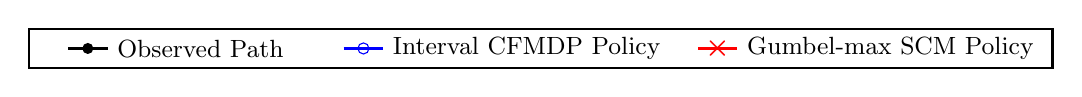
\begin{tikzpicture}[scale=1.0, every node/.style={scale=1.0}]
            \draw[thick, black] (-3, -0.25) rectangle (10, 0.25);
            %
            \draw[black, line width=1pt] (-2.5, 0.0) -- (-2,0.0);
            \fill[black] (-2.25,0.0) circle (2pt); %
            \node[right] at (-2,0.0) {\small Observed Path};
            
            %
            \draw[blue, line width=1pt] (1.0,0.0) -- (1.5,0.0);
            \node[draw=blue, circle, minimum size=4pt, inner sep=0pt] at (1.25,0.0) {}; %
            \node[right] at (1.5,0.0) {\small Interval CFMDP Policy};
            
            %
            \draw[red, line width=1pt] (5.5,0) -- (6,0);
            \node[red] at (5.75,0) {$\boldsymbol{\times}$}; %
            \node[right] at (6,0) {\small Gumbel-max SCM Policy};
        \end{tikzpicture}
    }\\
    %
    \subfigure[\footnotesize Lowest cumulative reward: Interval CFMDP ($312$), Gumbel-max SCM ($312$)]{%
        \resizebox{0.76\columnwidth}{!}{
             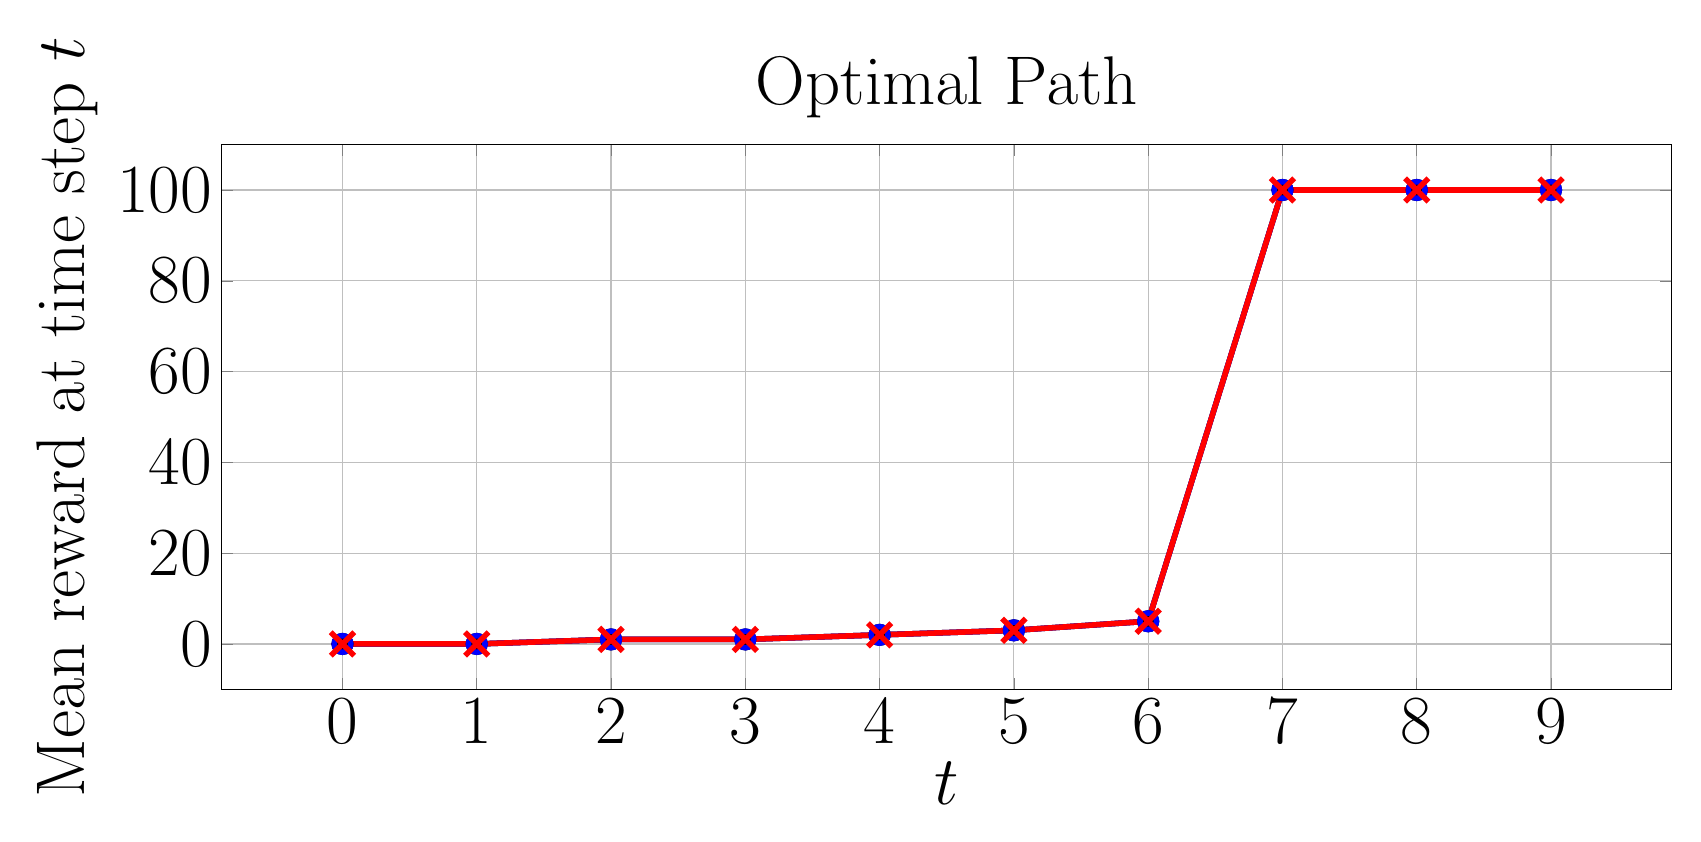
\begin{tikzpicture}
                \begin{axis}[
                    xlabel={$t$},
                    ylabel={Mean reward at time step $t$},
                    title={Optimal Path},
                    grid=both,
                    width=20cm, height=8.5cm,
                    every axis/.style={font=\Huge},
                    %
                ]
                \addplot[
                    color=black, %
                    mark=*, %
                    line width=2pt,
                    mark size=3pt,
                    error bars/.cd,
                    y dir=both, %
                    y explicit, %
                    error bar style={line width=1pt,solid},
                    error mark options={line width=1pt,mark size=4pt,rotate=90}
                ]
                coordinates {
                    (0, 0.0)  +- (0, 0.0)
                    (1, 0.0)  +- (0, 0.0) 
                    (2, 1.0)  +- (0, 0.0) 
                    (3, 1.0)  +- (0, 0.0)
                    (4, 2.0)  +- (0, 0.0)
                    (5, 3.0) +- (0, 0.0)
                    (6, 5.0) +- (0, 0.0)
                    (7, 100.0) +- (0, 0.0)
                    (8, 100.0) +- (0, 0.0)
                    (9, 100.0) +- (0, 0.0)
                };
                %
                \addplot[
                    color=blue, %
                    mark=o, %
                    line width=2pt,
                    mark size=3pt,
                    error bars/.cd,
                    y dir=both, %
                    y explicit, %
                    error bar style={line width=1pt,solid},
                    error mark options={line width=1pt,mark size=4pt,rotate=90}
                ]
                 coordinates {
                    (0, 0.0)  +- (0, 0.0)
                    (1, 0.0)  +- (0, 0.0) 
                    (2, 1.0)  +- (0, 0.0) 
                    (3, 1.0)  +- (0, 0.0)
                    (4, 2.0)  +- (0, 0.0)
                    (5, 3.0) +- (0, 0.0)
                    (6, 5.0) +- (0, 0.0)
                    (7, 100.0) +- (0, 0.0)
                    (8, 100.0) +- (0, 0.0)
                    (9, 100.0) +- (0, 0.0)
                };
                %
                \addplot[
                    color=red, %
                    mark=x, %
                    line width=2pt,
                    mark size=6pt,
                    error bars/.cd,
                    y dir=both, %
                    y explicit, %
                    error bar style={line width=1pt,solid},
                    error mark options={line width=1pt,mark size=4pt,rotate=90}
                ]
                coordinates {
                    (0, 0.0)  +- (0, 0.0)
                    (1, 0.0)  +- (0, 0.0) 
                    (2, 1.0)  +- (0, 0.0) 
                    (3, 1.0)  +- (0, 0.0)
                    (4, 2.0)  +- (0, 0.0)
                    (5, 3.0) +- (0, 0.0)
                    (6, 5.0) +- (0, 0.0)
                    (7, 100.0) +- (0, 0.0)
                    (8, 100.0) +- (0, 0.0)
                    (9, 100.0) +- (0, 0.0)
                };
                \end{axis}
            \end{tikzpicture}
         }
    }
    \hspace{1cm}
    \subfigure[\footnotesize Lowest cumulative reward: Interval CFMDP ($19$), Gumbel-max SCM ($-88$)]{%
         \resizebox{0.76\columnwidth}{!}{
            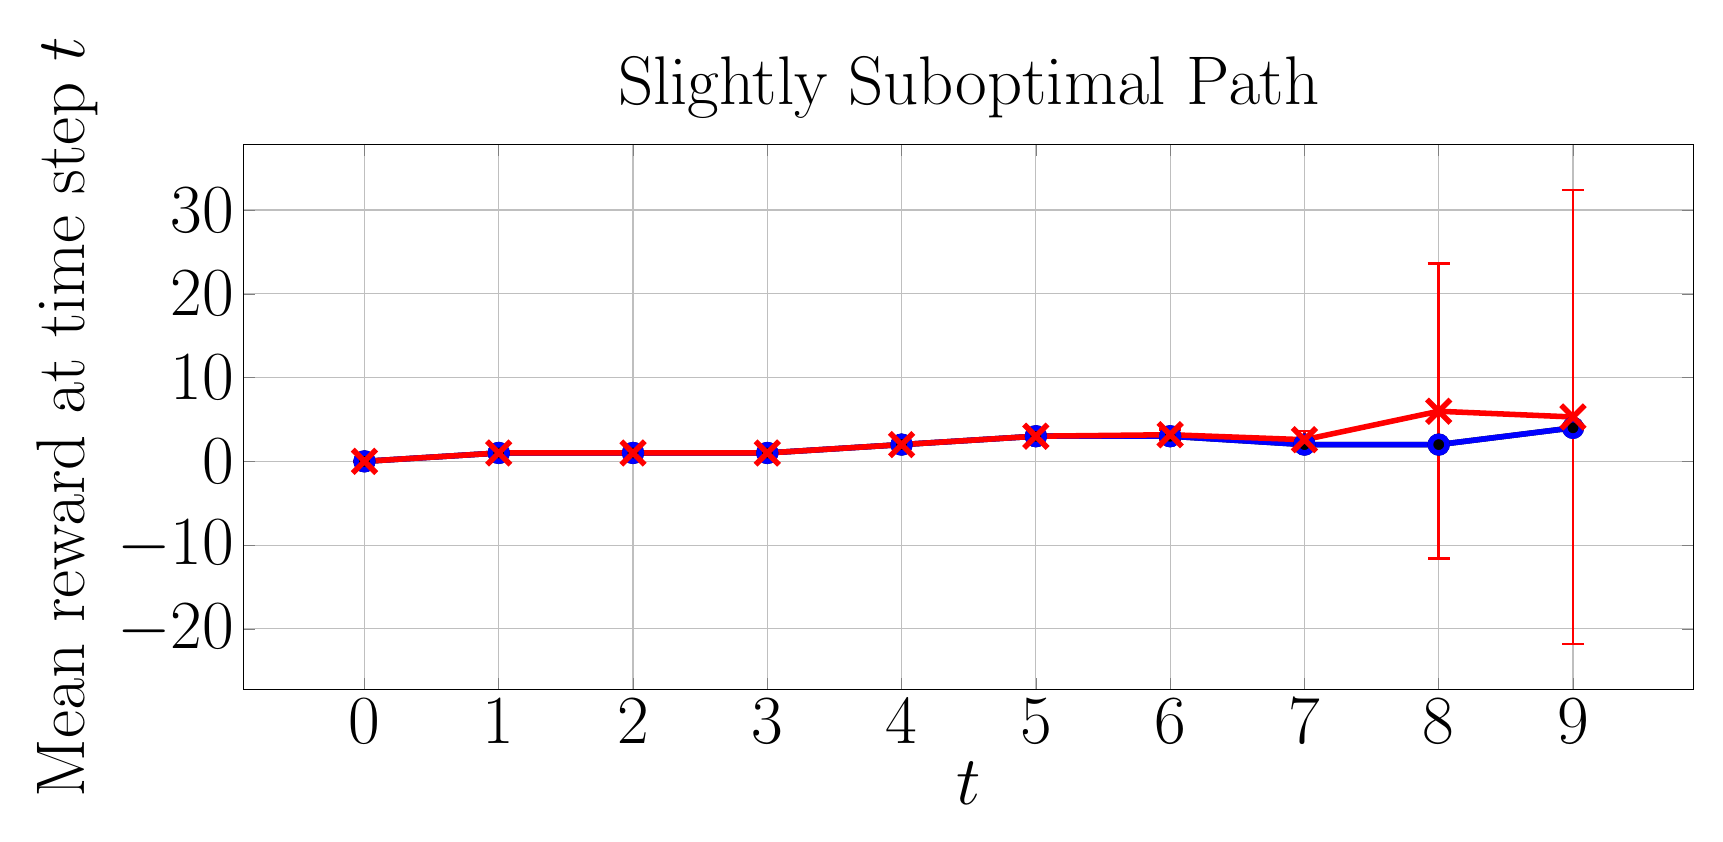
\begin{tikzpicture}
                \begin{axis}[
                    xlabel={$t$},
                    ylabel={Mean reward at time step $t$},
                    title={Slightly Suboptimal Path},
                    grid=both,
                    width=20cm, height=8.5cm,
                    every axis/.style={font=\Huge},
                    %
                ]
                \addplot[
                    color=black, %
                    mark=*, %
                    line width=2pt,
                    mark size=3pt,
                    error bars/.cd,
                    y dir=both, %
                    y explicit, %
                    error bar style={line width=1pt,solid},
                    error mark options={line width=1pt,mark size=4pt,rotate=90}
                ]
              coordinates {
                    (0, 0.0)  +- (0, 0.0)
                    (1, 1.0)  +- (0, 0.0) 
                    (2, 1.0)  +- (0, 0.0) 
                    (3, 1.0)  +- (0, 0.0)
                    (4, 2.0)  +- (0, 0.0)
                    (5, 3.0) +- (0, 0.0)
                    (6, 3.0) +- (0, 0.0)
                    (7, 2.0) +- (0, 0.0)
                    (8, 2.0) +- (0, 0.0)
                    (9, 4.0) +- (0, 0.0)
                };
                %
                \addplot[
                    color=blue, %
                    mark=o, %
                    line width=2pt,
                    mark size=3pt,
                    error bars/.cd,
                    y dir=both, %
                    y explicit, %
                    error bar style={line width=1pt,solid},
                    error mark options={line width=1pt,mark size=4pt,rotate=90}
                ]
              coordinates {
                    (0, 0.0)  +- (0, 0.0)
                    (1, 1.0)  +- (0, 0.0) 
                    (2, 1.0)  +- (0, 0.0) 
                    (3, 1.0)  +- (0, 0.0)
                    (4, 2.0)  +- (0, 0.0)
                    (5, 3.0) +- (0, 0.0)
                    (6, 3.0) +- (0, 0.0)
                    (7, 2.0) +- (0, 0.0)
                    (8, 2.0) +- (0, 0.0)
                    (9, 4.0) +- (0, 0.0)
                };
                %
                \addplot[
                    color=red, %
                    mark=x, %
                    line width=2pt,
                    mark size=6pt,
                    error bars/.cd,
                    y dir=both, %
                    y explicit, %
                    error bar style={line width=1pt,solid},
                    error mark options={line width=1pt,mark size=4pt,rotate=90}
                ]
                coordinates {
                    (0, 0.0)  +- (0, 0.0)
                    (1, 1.0)  +- (0, 0.0) 
                    (2, 1.0)  +- (0, 0.0) 
                    (3, 1.0)  +- (0, 0.0)
                    (4, 2.0)  += (0, 0.0)
                    (5, 3.0)  += (0, 0.0)
                    (6, 3.17847) += (0, 0.62606746) -= (0, 0.62606746)
                    (7, 2.5832885) += (0, 1.04598233) -= (0, 1.04598233)
                    (8, 5.978909) += (0, 17.60137623) -= (0, 17.60137623)
                    (9, 5.297059) += (0, 27.09227512) -= (0, 27.09227512)
                };
                \end{axis}
            \end{tikzpicture}
         }
    }\\[-1.5pt]
    \subfigure[\footnotesize Lowest cumulative reward: Interval CFMDP ($14$), Gumbel-max SCM ($-598$)]{%
         \resizebox{0.76\columnwidth}{!}{
             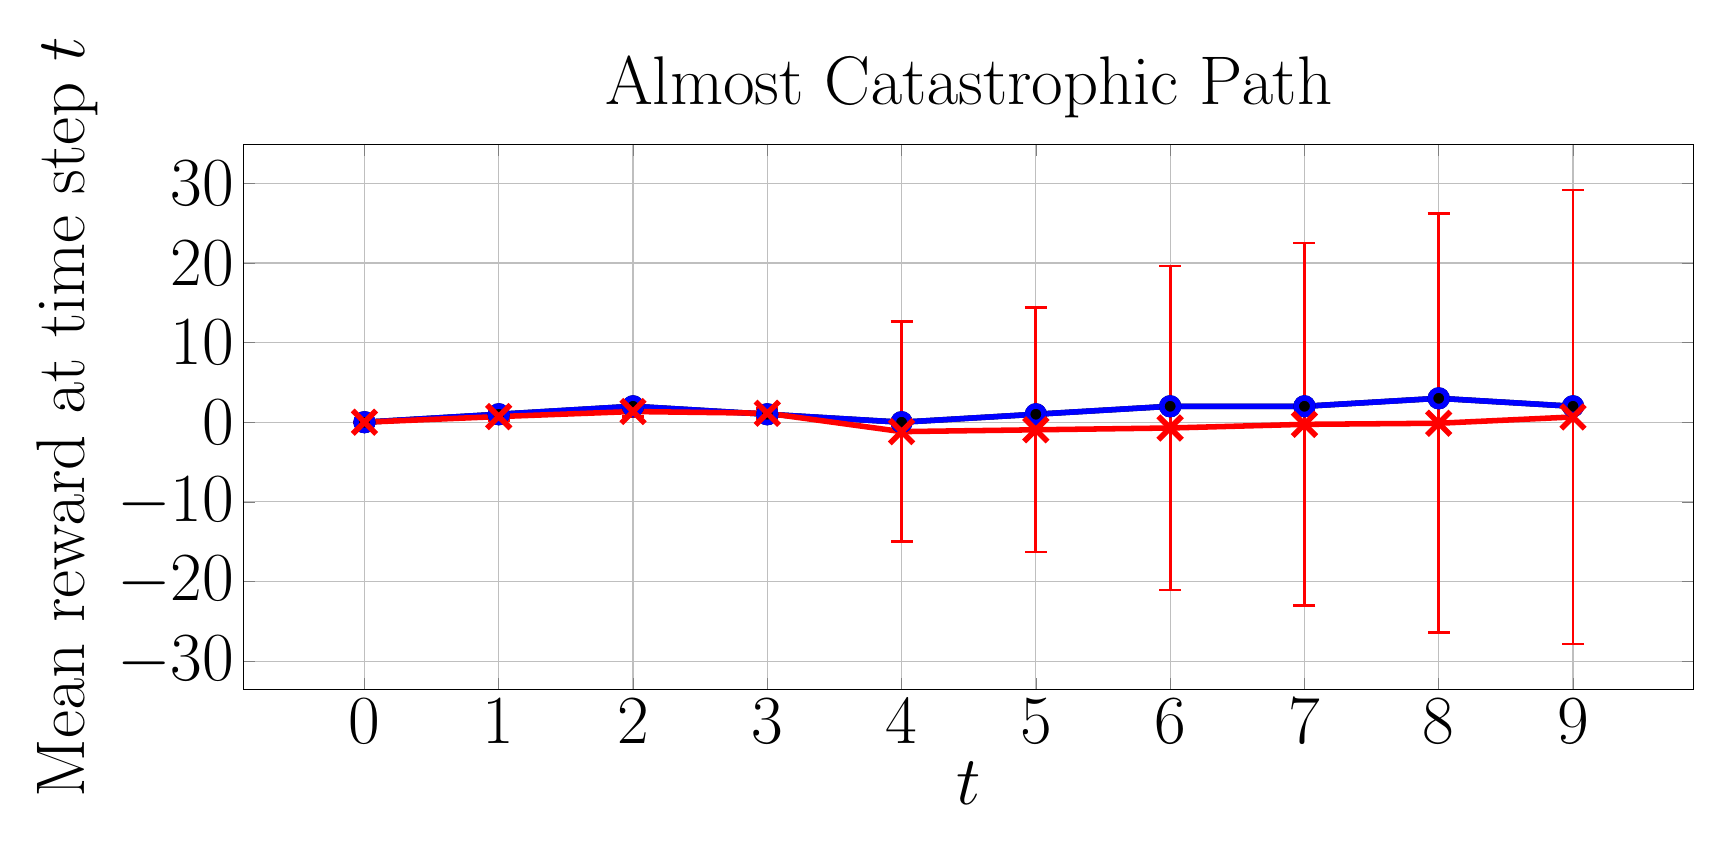
\begin{tikzpicture}
                \begin{axis}[
                    xlabel={$t$},
                    ylabel={Mean reward at time step $t$},
                    title={Almost Catastrophic Path},
                    grid=both,
                    width=20cm, height=8.5cm,
                    every axis/.style={font=\Huge},
                    %
                ]
                \addplot[
                    color=black, %
                    mark=*, %
                    line width=2pt,
                    mark size=3pt,
                    error bars/.cd,
                    y dir=both, %
                    y explicit, %
                    error bar style={line width=1pt,solid},
                    error mark options={line width=1pt,mark size=4pt,rotate=90}
                ]
                coordinates {
                    (0, 0.0)  +- (0, 0.0)
                    (1, 1.0)  +- (0, 0.0) 
                    (2, 2.0)  +- (0, 0.0) 
                    (3, 1.0)  +- (0, 0.0)
                    (4, 0.0)  +- (0, 0.0)
                    (5, 1.0) +- (0, 0.0)
                    (6, 2.0) +- (0, 0.0)
                    (7, 2.0) +- (0, 0.0)
                    (8, 3.0) +- (0, 0.0)
                    (9, 2.0) +- (0, 0.0)
                };
                %
                \addplot[
                    color=blue, %
                    mark=o, %
                    line width=2pt,
                    mark size=3pt,
                    error bars/.cd,
                    y dir=both, %
                    y explicit, %
                    error bar style={line width=1pt,solid},
                    error mark options={line width=1pt,mark size=4pt,rotate=90}
                ]
                coordinates {
                    (0, 0.0)  +- (0, 0.0)
                    (1, 1.0)  +- (0, 0.0) 
                    (2, 2.0)  +- (0, 0.0) 
                    (3, 1.0)  +- (0, 0.0)
                    (4, 0.0)  +- (0, 0.0)
                    (5, 1.0) +- (0, 0.0)
                    (6, 2.0) +- (0, 0.0)
                    (7, 2.0) +- (0, 0.0)
                    (8, 3.0) +- (0, 0.0)
                    (9, 2.0) +- (0, 0.0)
                };
                %
                \addplot[
                    color=red, %
                    mark=x, %
                    line width=2pt,
                    mark size=6pt,
                    error bars/.cd,
                    y dir=both, %
                    y explicit, %
                    error bar style={line width=1pt,solid},
                    error mark options={line width=1pt,mark size=4pt,rotate=90}
                ]
                coordinates {
                    (0, 0.0)  +- (0, 0.0)
                    (1, 0.7065655)  +- (0, 0.4553358) 
                    (2, 1.341673)  +- (0, 0.67091621) 
                    (3, 1.122926)  +- (0, 0.61281824)
                    (4, -1.1821935)  +- (0, 13.82444042)
                    (5, -0.952399)  +- (0, 15.35195457)
                    (6, -0.72672) +- (0, 20.33508414)
                    (7, -0.268983) +- (0, 22.77861454)
                    (8, -0.1310835) +- (0, 26.31013314)
                    (9, 0.65806) +- (0, 28.50670214)
                };
                %
            %
            %
            %
            %
            %
            %
            %
            %
            %
            %
            %
            %
            %
            %
            %
            %
            %
            %
                \end{axis}
            \end{tikzpicture}
         }
    }
    \hspace{1cm}
    \subfigure[\footnotesize Lowest cumulative reward: Interval CFMDP ($-698$), Gumbel-max SCM ($-698$)]{%
         \resizebox{0.76\columnwidth}{!}{
            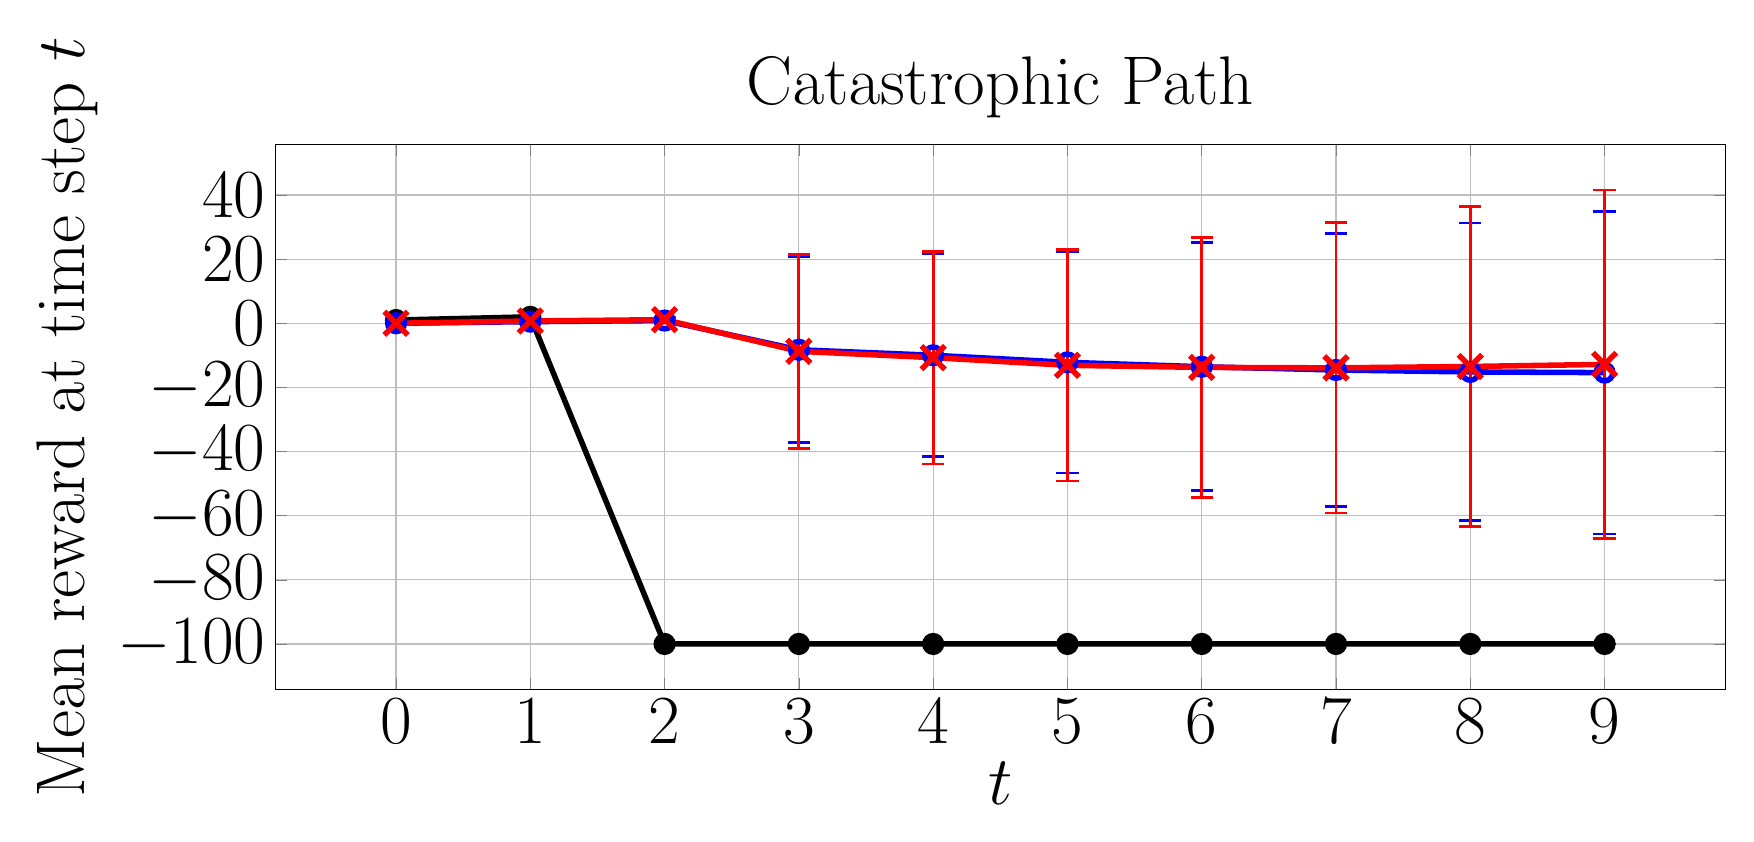
\begin{tikzpicture}
                \begin{axis}[
                    xlabel={$t$},
                    ylabel={Mean reward at time step $t$},
                    title={Catastrophic Path},
                    grid=both,
                    width=20cm, height=8.5cm,
                    every axis/.style={font=\Huge},
                    %
                ]
                \addplot[
                    color=black, %
                    mark=*, %
                    line width=2pt,
                    mark size=3pt,
                    error bars/.cd,
                    y dir=both, %
                    y explicit, %
                    error bar style={line width=1pt,solid},
                    error mark options={line width=1pt,mark size=4pt,rotate=90}
                ]
                coordinates {
                    (0, 1.0)  +- (0, 0.0)
                    (1, 2.0)  +- (0, 0.0) 
                    (2, -100.0)  +- (0, 0.0) 
                    (3, -100.0)  +- (0, 0.0)
                    (4, -100.0)  +- (0, 0.0)
                    (5, -100.0) +- (0, 0.0)
                    (6, -100.0) +- (0, 0.0)
                    (7, -100.0) +- (0, 0.0)
                    (8, -100.0) +- (0, 0.0)
                    (9, -100.0) +- (0, 0.0)
                };
                %
                \addplot[
                    color=blue, %
                    mark=o, %
                    line width=2pt,
                    mark size=3pt,
                    error bars/.cd,
                    y dir=both, %
                    y explicit, %
                    error bar style={line width=1pt,solid},
                    error mark options={line width=1pt,mark size=4pt,rotate=90}
                ]
                coordinates {
                    (0, 0.0)  +- (0, 0.0)
                    (1, 0.504814)  +- (0, 0.49997682) 
                    (2, 0.8439835)  +- (0, 0.76831917) 
                    (3, -8.2709165)  +- (0, 28.93656754)
                    (4, -9.981082)  +- (0, 31.66825363)
                    (5, -12.1776325) +- (0, 34.53463233)
                    (6, -13.556076) +- (0, 38.62845372)
                    (7, -14.574418) +- (0, 42.49603359)
                    (8, -15.1757075) +- (0, 46.41913968)
                    (9, -15.3900395) +- (0, 50.33563368)
                };
                %
                \addplot[
                    color=red, %
                    mark=x, %
                    line width=2pt,
                    mark size=6pt,
                    error bars/.cd,
                    y dir=both, %
                    y explicit, %
                    error bar style={line width=1pt,solid},
                    error mark options={line width=1pt,mark size=4pt,rotate=90}
                ]
                coordinates {
                    (0, 0.0)  +- (0, 0.0)
                    (1, 0.701873)  +- (0, 0.45743556) 
                    (2, 1.1227805)  +- (0, 0.73433129) 
                    (3, -8.7503255)  +- (0, 30.30257976)
                    (4, -10.722092)  +- (0, 33.17618589)
                    (5, -13.10721)  +- (0, 36.0648089)
                    (6, -13.7631645) +- (0, 40.56553451)
                    (7, -13.909043) +- (0, 45.23829402)
                    (8, -13.472517) +- (0, 49.96270296)
                    (9, -12.8278835) +- (0, 54.38618735)
                };
                %
            %
            %
            %
            %
            %
            %
            %
            %
            %
            %
            %
            %
            %
            %
            %
            %
            %
            %
                \end{axis}
            \end{tikzpicture}
         }
    }
    \caption{Average instant reward of CF paths induced by policies on GridWorld $p=0.4$.}
    \label{fig: reward p=0.4}
\end{figure*}

\subsection{Experimental Setup}
To compare policy performance, we measure the average rewards of counterfactual paths induced by our policy and the Gumbel-max policy by uniformly sampling $200$ counterfactual MDPs from the ICFMDP and generating $10,000$ counterfactual paths over each sampled CFMDP. \jl{Since the interval CFMDP depends on the observed path, we select $4$  paths of varying optimality to evaluate how the observed path impacts the performance of both policies: an optimal path, a slightly suboptimal path that could reach the optimal reward with a few changes, a catastrophic path that enters a catastrophic, terminal state with low reward, and an almost catastrophic path that was close to entering a catastrophic state.} When measuring the average probability bound widths and execution time needed to generate the ICFMDPs, we averaged over $20$ randomly generated observed paths
\footnote{Further training details are provided in Appendix \ref{app: training details}, and the code is provided at \href{https://github.com/ddv-lab/robust-cf-inference-in-MDPs}{https://github.com/ddv-lab/robust-cf-inference-in-MDPs}
%
%
.}.

\subsection{GridWorld}
\jl{The GridWorld MDP is a $4 \times 4$ grid where an agent must navigate from the top-left corner to the goal state in the bottom-right corner, avoiding a dangerous terminal state in the centre. At each time step, the agent can move up, down, left, or right, but there is a small probability (controlled by hyper-parameter $p$) of moving in an unintended direction. As the agent nears the goal, the reward for each state increases, culminating in a reward of $+100$ for reaching the goal. Entering the dangerous state results in a penalty of $-100$. We use two versions of GridWorld: a less stochastic version with $p=0.9$ (i.e., $90$\% chance of moving in the chosen direction) and a more stochastic version with $p=0.4$.}

\paragraph{GridWorld ($p=0.9$)}
When $p=0.9$, the counterfactual probability bounds are typically narrow (see Table \ref{tab:nonzero_probs} for average measurements). Consequently, as shown in Figure \ref{fig: reward p=0.9}, both policies are nearly identical and perform similarly well across the optimal, slightly suboptimal, and catastrophic paths.
%
However, for the almost catastrophic path, the interval CFMDP path is more conservative and follows the observed path more closely (as this is where the probability bounds are narrowest), which typically requires one additional step to reach the goal state than the Gumbel-max SCM policy.
%

\paragraph{GridWorld ($p=0.4$)}
\jl{When $p=0.4$, the GridWorld environment becomes more uncertain, increasing the risk of entering the dangerous state even if correct actions are chosen. Thus, as shown in Figure \ref{fig: reward p=0.4}, the interval CFMDP policy adopts a more conservative approach, avoiding deviation from the observed policy if it cannot guarantee higher counterfactual rewards (see the slightly suboptimal and almost catastrophic paths), whereas the Gumbel-max SCM is inconsistent: it can yield higher rewards, but also much lower rewards, reflected in the wide error bars.} For the catastrophic path, both policies must deviate from the observed path to achieve a higher reward and, in this case, perform similarly.
%
%
%
%
\subsection{Sepsis}
The Sepsis MDP \citep{oberst2019counterfactual} simulates trajectories of Sepsis patients. Each state consists of four vital signs (heart rate, blood pressure, oxygen concentration, and glucose levels), categorised as low, normal, or high.
and three treatments that can be toggled on/off at each time step (8 actions in total). Unlike \citet{oberst2019counterfactual}, we scale rewards based on the number of out-of-range vital signs, between $-1000$ (patient dies) and $1000$ (patient discharged). \jl{Like the GridWorld $p=0.4$ experiment, the Sepsis MDP is highly uncertain, as many states are equally likely to lead to optimal and poor outcomes. Thus, as shown in Figure \ref{fig: reward sepsis}, both policies follow the observed optimal and almost catastrophic paths to guarantee rewards are no worse than the observation.} However, improving the catastrophic path requires deviating from the observation. Here, the Gumbel-max SCM policy, on average, performs better than the interval CFMDP policy. But, since both policies have lower bounds clipped at $-1000$, neither policy reliably improves over the observation. In contrast, for the slightly suboptimal path, the interval CFMDP policy performs significantly better, shown by its higher lower bounds. 
Moreover, in these two cases, the worst-case counterfactual path generated by the interval CFMDP policy is better than that of the Gumbel-max SCM policy,
indicating its greater robustness.
%
\begin{figure*}
    \centering
     \resizebox{0.6\textwidth}{!}{
        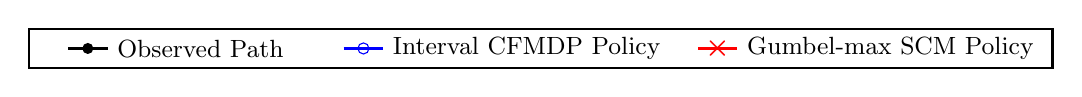
\begin{tikzpicture}[scale=1.0, every node/.style={scale=1.0}]
            \draw[thick, black] (-3, -0.25) rectangle (10, 0.25);
            %
            \draw[black, line width=1pt] (-2.5, 0.0) -- (-2,0.0);
            \fill[black] (-2.25,0.0) circle (2pt); %
            \node[right] at (-2,0.0) {\small Observed Path};
            
            %
            \draw[blue, line width=1pt] (1.0,0.0) -- (1.5,0.0);
            \node[draw=blue, circle, minimum size=4pt, inner sep=0pt] at (1.25,0.0) {}; %
            \node[right] at (1.5,0.0) {\small Interval CFMDP Policy};
            
            %
            \draw[red, line width=1pt] (5.5,0) -- (6,0);
            \node[red] at (5.75,0) {$\boldsymbol{\times}$}; %
            \node[right] at (6,0) {\small Gumbel-max SCM Policy};
        \end{tikzpicture}
    }\\
    \subfigure[\footnotesize Lowest cumulative reward: Interval CFMDP ($8000$), Gumbel-max SCM ($8000$)]{%
         \resizebox{0.76\columnwidth}{!}{
             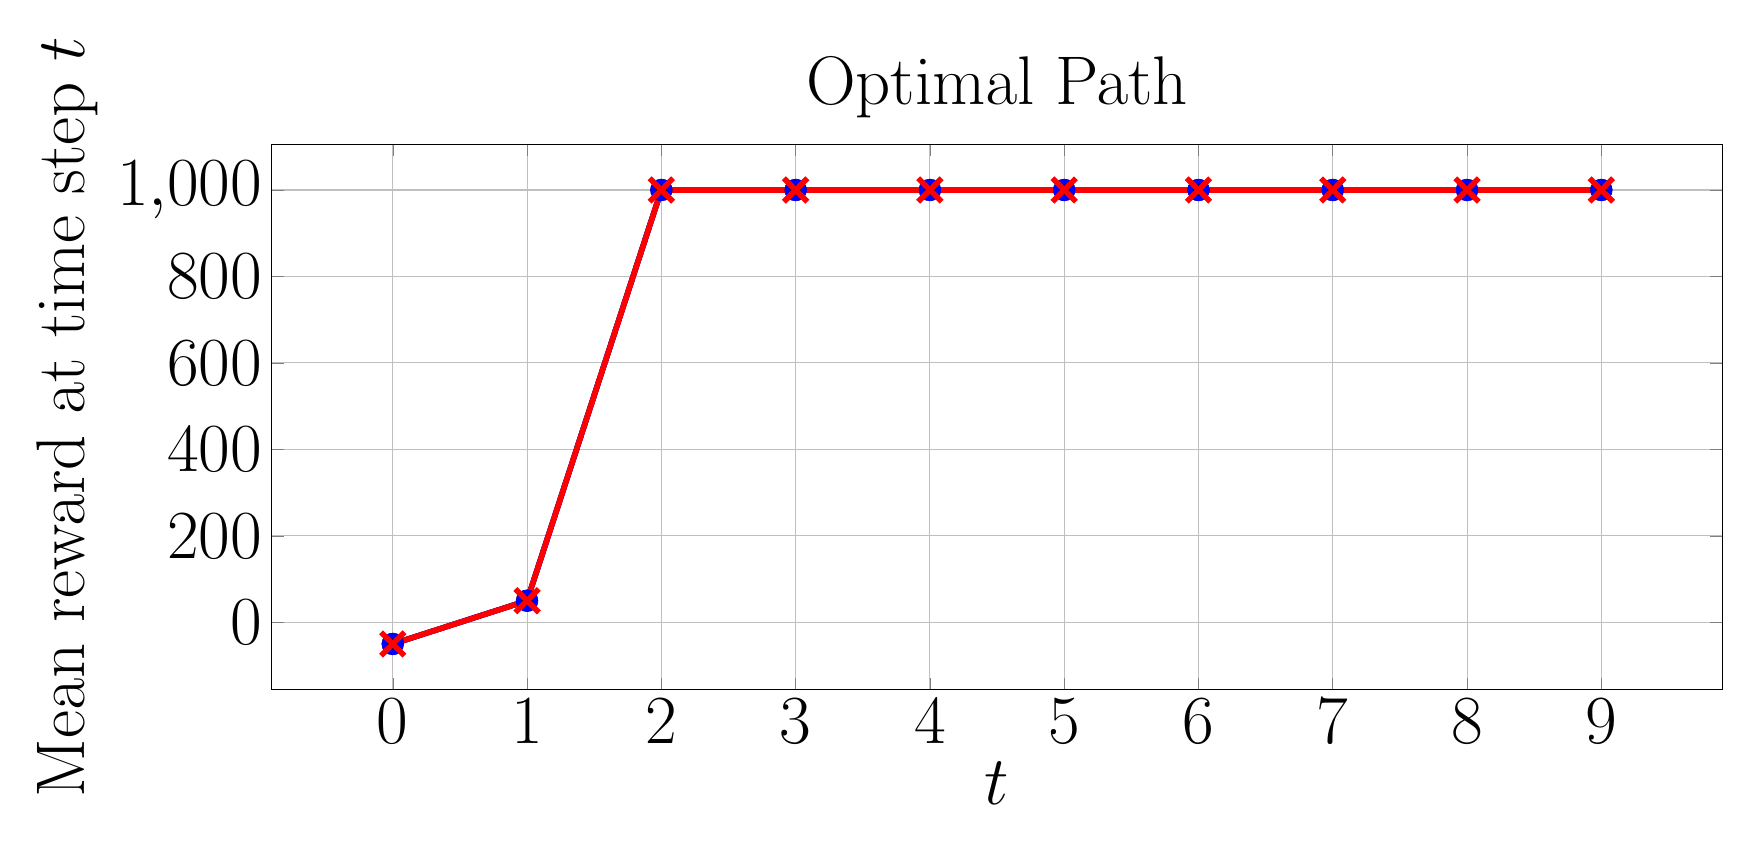
\begin{tikzpicture}
                \begin{axis}[
                    xlabel={$t$},
                    ylabel={Mean reward at time step $t$},
                    title={Optimal Path},
                    grid=both,
                    width=20cm, height=8.5cm,
                    every axis/.style={font=\Huge},
                    %
                ]
                \addplot[
                    color=black, %
                    mark=*, %
                    line width=2pt,
                    mark size=3pt,
                ]
                coordinates {
                    (0, -50.0)
                    (1, 50.0)
                    (2, 1000.0)
                    (3, 1000.0)
                    (4, 1000.0)
                    (5, 1000.0)
                    (6, 1000.0)
                    (7, 1000.0)
                    (8, 1000.0)
                    (9, 1000.0)
                };
                %
                \addplot[
                    color=blue, %
                    mark=o, %
                    line width=2pt,
                    mark size=3pt,
                    error bars/.cd,
                    y dir=both, %
                    y explicit, %
                    error bar style={line width=1pt,solid},
                    error mark options={line width=1pt,mark size=4pt,rotate=90}
                ]
                coordinates {
                    (0, -50.0)  +- (0, 0.0)
                    (1, 50.0)  +- (0, 0.0) 
                    (2, 1000.0)  +- (0, 0.0) 
                    (3, 1000.0)  +- (0, 0.0)
                    (4, 1000.0)  +- (0, 0.0)
                    (5, 1000.0) +- (0, 0.0)
                    (6, 1000.0) +- (0, 0.0)
                    (7, 1000.0) +- (0, 0.0)
                    (8, 1000.0) +- (0, 0.0)
                    (9, 1000.0) +- (0, 0.0)
                };
                %
                \addplot[
                    color=red, %
                    mark=x, %
                    line width=2pt,
                    mark size=6pt,
                    error bars/.cd,
                    y dir=both, %
                    y explicit, %
                    error bar style={line width=1pt,solid},
                    error mark options={line width=1pt,mark size=4pt,rotate=90}
                ]
                coordinates {
                    (0, -50.0)  +- (0, 0.0)
                    (1, 50.0)  +- (0, 0.0) 
                    (2, 1000.0)  +- (0, 0.0) 
                    (3, 1000.0)  +- (0, 0.0)
                    (4, 1000.0)  +- (0, 0.0)
                    (5, 1000.0) +- (0, 0.0)
                    (6, 1000.0) +- (0, 0.0)
                    (7, 1000.0) +- (0, 0.0)
                    (8, 1000.0) +- (0, 0.0)
                    (9, 1000.0) +- (0, 0.0)
                };
                %
                \end{axis}
            \end{tikzpicture}
         }
    }
    \hspace{1cm}
    \subfigure[\footnotesize Lowest cumulative reward: Interval CFMDP ($-5980$), Gumbel-max SCM ($-8000$)]{%
         \resizebox{0.76\columnwidth}{!}{
            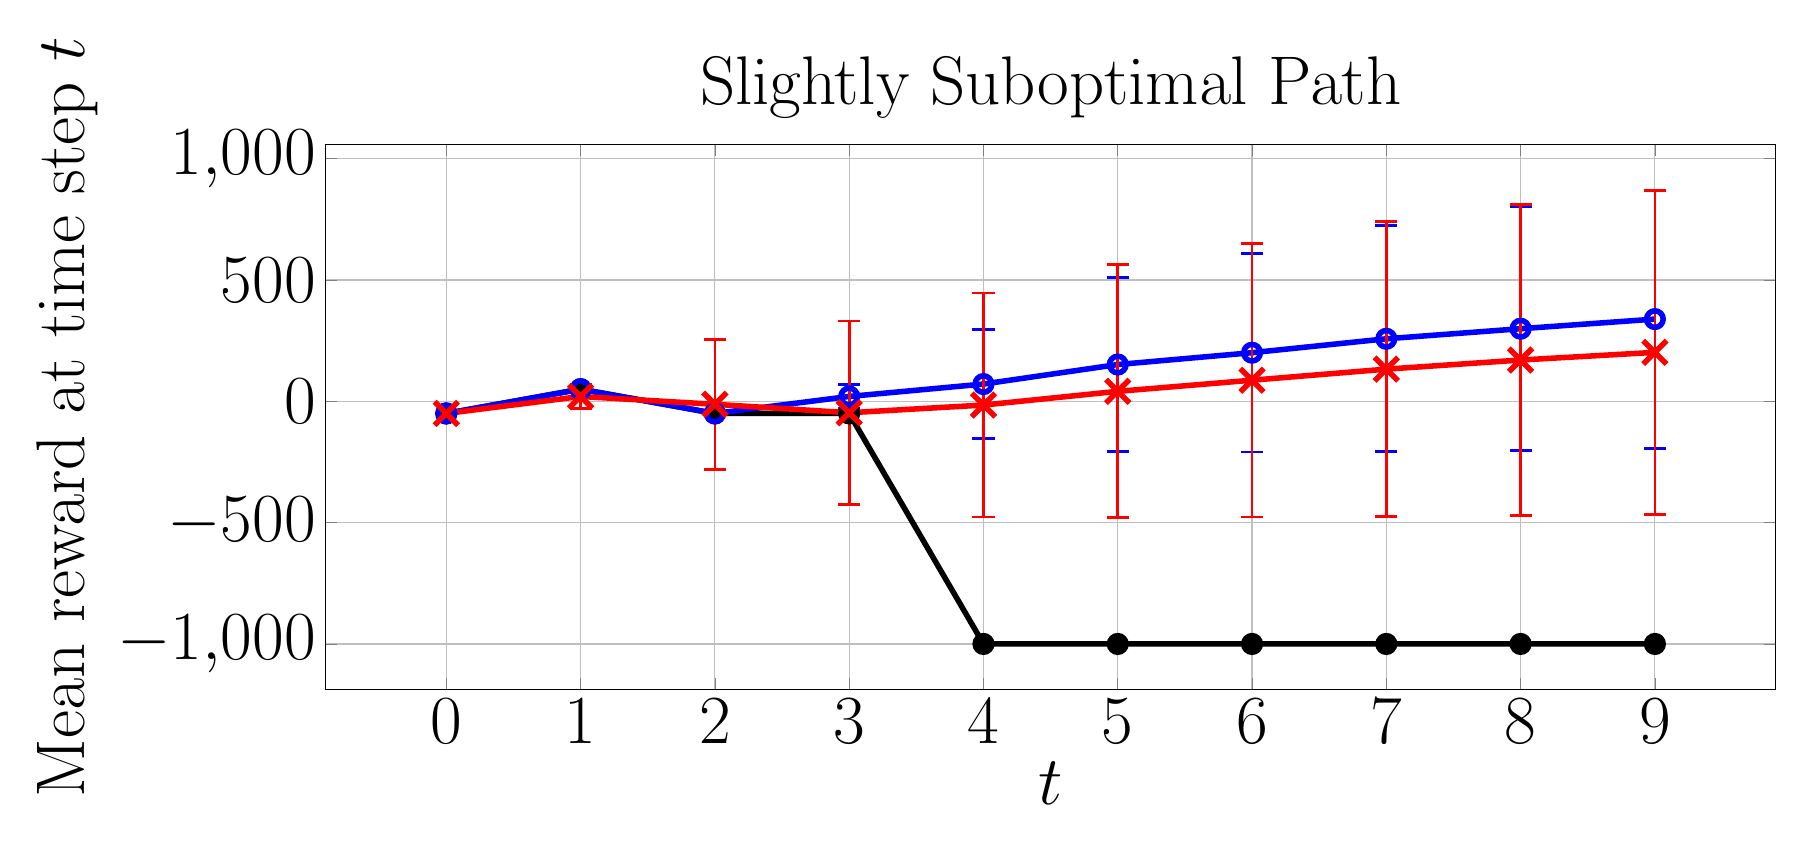
\begin{tikzpicture}
                \begin{axis}[
                    xlabel={$t$},
                    ylabel={Mean reward at time step $t$},
                    title={Slightly Suboptimal Path},
                    grid=both,
                    width=20cm, height=8.5cm,
                    every axis/.style={font=\Huge},
                    %
                ]
               \addplot[
                    color=black, %
                    mark=*, %
                    line width=2pt,
                    mark size=3pt,
                ]
                coordinates {
                    (0, -50.0)
                    (1, 50.0)
                    (2, -50.0)
                    (3, -50.0)
                    (4, -1000.0)
                    (5, -1000.0)
                    (6, -1000.0)
                    (7, -1000.0)
                    (8, -1000.0)
                    (9, -1000.0)
                };
                %
                \addplot[
                    color=blue, %
                    mark=o, %
                    line width=2pt,
                    mark size=3pt,
                    error bars/.cd,
                    y dir=both, %
                    y explicit, %
                    error bar style={line width=1pt,solid},
                    error mark options={line width=1pt,mark size=4pt,rotate=90}
                ]
                coordinates {
                    (0, -50.0)  +- (0, 0.0)
                    (1, 50.0)  +- (0, 0.0) 
                    (2, -50.0)  +- (0, 0.0) 
                    (3, 20.0631)  +- (0, 49.97539413)
                    (4, 71.206585)  +- (0, 226.02033693)
                    (5, 151.60797) +- (0, 359.23292559)
                    (6, 200.40593) +- (0, 408.86185176)
                    (7, 257.77948) +- (0, 466.10372804)
                    (8, 299.237465) +- (0, 501.82579506)
                    (9, 338.9129) +- (0, 532.06124996)
                };
                %
                \addplot[
                    color=red, %
                    mark=x, %
                    line width=2pt,
                    mark size=6pt,
                    error bars/.cd,
                    y dir=both, %
                    y explicit, %
                    error bar style={line width=1pt,solid},
                    error mark options={line width=1pt,mark size=4pt,rotate=90}
                ]
                coordinates {
                    (0, -50.0)  +- (0, 0.0)
                    (1, 20.00736)  +- (0, 49.99786741) 
                    (2, -12.282865)  +- (0, 267.598755) 
                    (3, -47.125995)  +- (0, 378.41755832)
                    (4, -15.381965)  +- (0, 461.77616558)
                    (5, 41.15459) +- (0, 521.53189262)
                    (6, 87.01595) +- (0, 564.22243126 )
                    (7, 132.62376) +- (0, 607.31338037)
                    (8, 170.168145) +- (0, 641.48013693)
                    (9, 201.813135) +- (0, 667.29441777)
                };
                %
                %
                %
                %
                %
                %
                %
                %
                %
                %
                %
                %
                %
                %
                %
                %
                %
                %
                %
                \end{axis}
            \end{tikzpicture}
         }
    }\\[-1.5pt]
    \subfigure[\footnotesize Lowest cumulative reward: Interval CFMDP ($100$), Gumbel-max SCM ($100$)]{%
         \resizebox{0.76\columnwidth}{!}{
             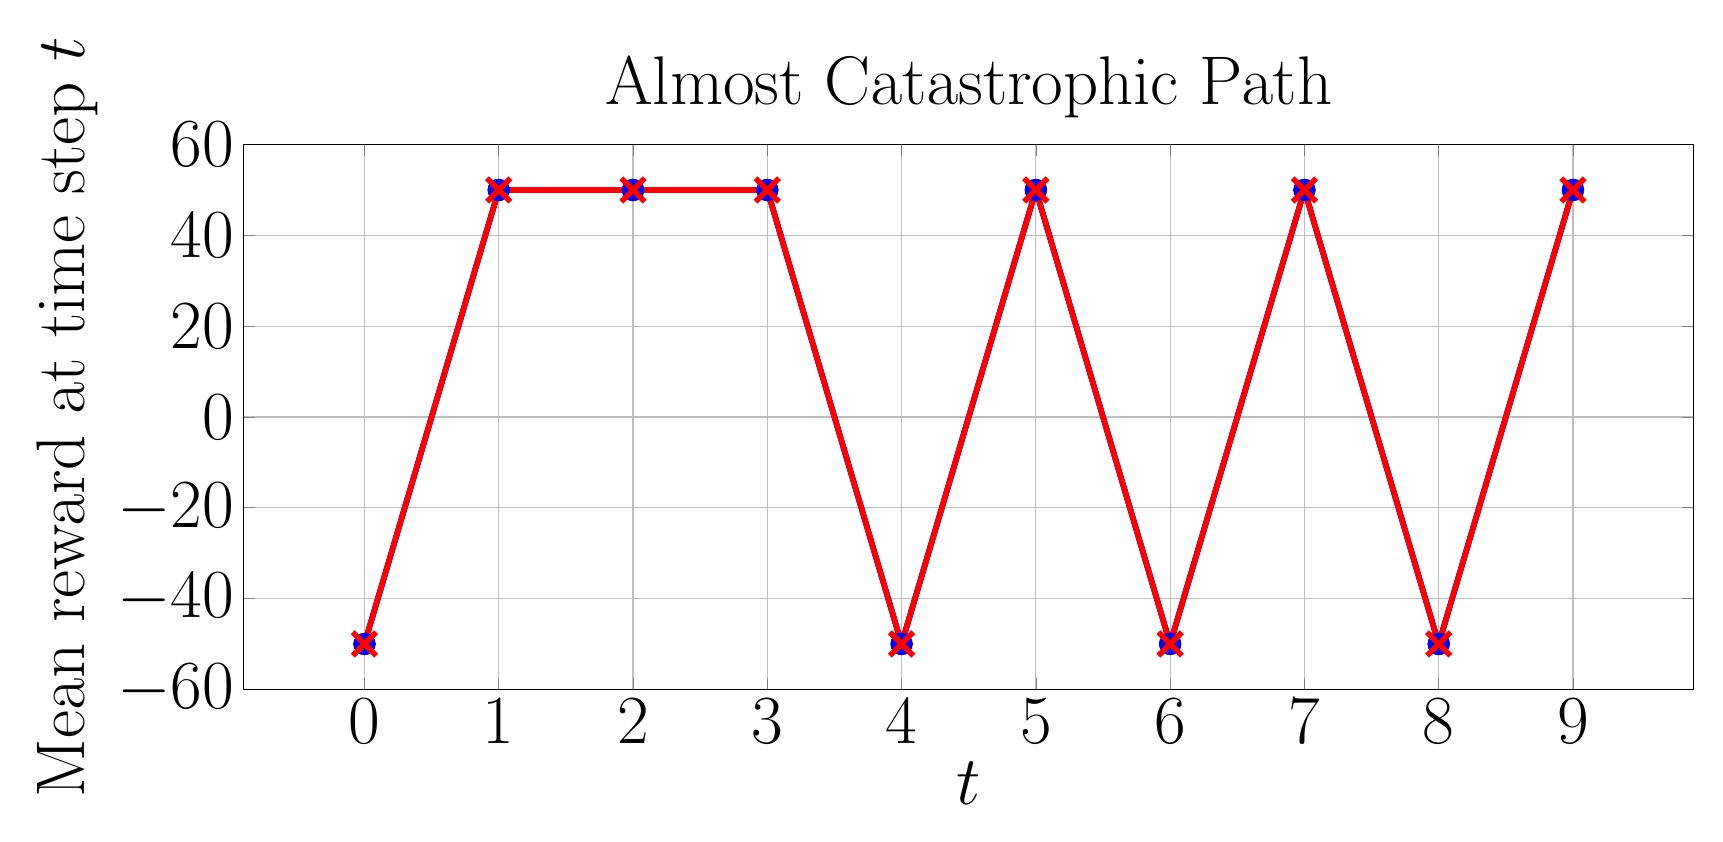
\begin{tikzpicture}
                \begin{axis}[
                    xlabel={$t$},
                    ylabel={Mean reward at time step $t$},
                    title={Almost Catastrophic Path},
                    grid=both,
                    every axis/.style={font=\Huge},
                    width=20cm, height=8.5cm,
                    %
                ]
               \addplot[
                    color=black, %
                    mark=*, %
                    line width=2pt,
                    mark size=3pt,
                ]
                coordinates {
                    (0, -50.0)
                    (1, 50.0)
                    (2, 50.0)
                    (3, 50.0)
                    (4, -50.0)
                    (5, 50.0)
                    (6, -50.0)
                    (7, 50.0)
                    (8, -50.0)
                    (9, 50.0)
                };
                %
                %
                \addplot[
                    color=blue, %
                    mark=o, %
                    line width=2pt,
                    mark size=3pt,
                    error bars/.cd,
                    y dir=both, %
                    y explicit, %
                    error bar style={line width=1pt,solid},
                    error mark options={line width=1pt,mark size=4pt,rotate=90}
                ]
                coordinates {
                    (0, -50.0)  +- (0, 0.0)
                    (1, 50.0)  +- (0, 0.0) 
                    (2, 50.0)  +- (0, 0.0) 
                    (3, 50.0)  +- (0, 0.0)
                    (4, -50.0)  +- (0, 0.0)
                    (5, 50.0) +- (0, 0.0)
                    (6, -50.0) +- (0, 0.0)
                    (7, 50.0) +- (0, 0.0)
                    (8, -50.0) +- (0, 0.0)
                    (9, 50.0) +- (0, 0.0)
                };
                %
                \addplot[
                    color=red, %
                    mark=x, %
                    line width=2pt,
                    mark size=6pt,
                    error bars/.cd,
                    y dir=both, %
                    y explicit, %
                    error bar style={line width=1pt,solid},
                    error mark options={line width=1pt,mark size=4pt,rotate=90}
                ]
                coordinates {
                    (0, -50.0)  +- (0, 0.0)
                    (1, 50.0)  +- (0, 0.0) 
                    (2, 50.0)  +- (0, 0.0) 
                    (3, 50.0)  +- (0, 0.0)
                    (4, -50.0)  +- (0, 0.0)
                    (5, 50.0) +- (0, 0.0)
                    (6, -50.0) +- (0, 0.0)
                    (7, 50.0) +- (0, 0.0)
                    (8, -50.0) +- (0, 0.0)
                    (9, 50.0) +- (0, 0.0)
                };
                %
                %
                %
                %
                %
                %
                %
                %
                %
                %
                %
                %
                %
                %
                %
                %
                %
                %
                %
                \end{axis}
            \end{tikzpicture}
         }
    }
    \hspace{1cm}
    \subfigure[\footnotesize Lowest cumulative reward: Interval CFMDP ($-7150$), Gumbel-max SCM ($-9050$)]{%
         \resizebox{0.76\columnwidth}{!}{
            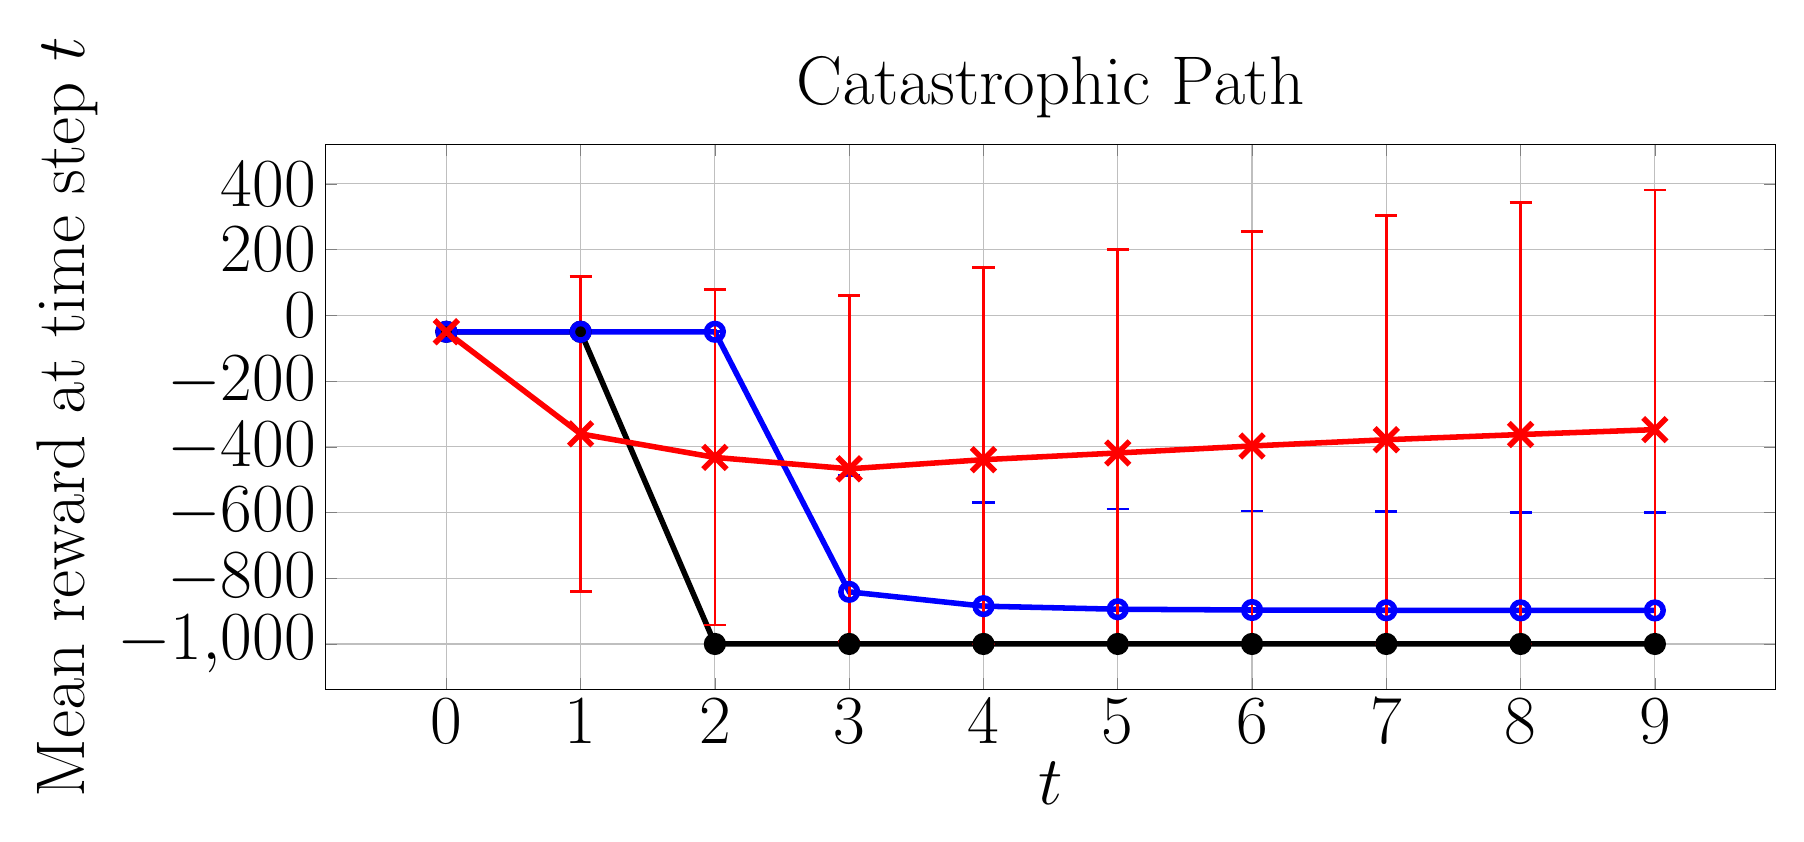
\begin{tikzpicture}
                \begin{axis}[
                    xlabel={$t$},
                    ylabel={Mean reward at time step $t$},
                    title={Catastrophic Path},
                    grid=both,
                    width=20cm, height=8.5cm,
                    every axis/.style={font=\Huge},
                    %
                ]
               \addplot[
                    color=black, %
                    mark=*, %
                    line width=2pt,
                    mark size=3pt,
                ]
                coordinates {
                    (0, -50.0)
                    (1, -50.0)
                    (2, -1000.0)
                    (3, -1000.0)
                    (4, -1000.0)
                    (5, -1000.0)
                    (6, -1000.0)
                    (7, -1000.0)
                    (8, -1000.0)
                    (9, -1000.0)
                };
                %
                %
                \addplot[
                    color=blue, %
                    mark=o, %
                    line width=2pt,
                    mark size=3pt,
                    error bars/.cd,
                    y dir=both, %
                    y explicit, %
                    error bar style={line width=1pt,solid},
                    error mark options={line width=1pt,mark size=4pt,rotate=90}
                ]
                coordinates {
                    (0, -50.0)  +- (0, 0.0)
                    (1, -50.0)  +- (0, 0.0) 
                    (2, -50.0)  +- (0, 0.0) 
                    (3, -841.440725)  += (0, 354.24605512) -= (0, 158.559275)
                    (4, -884.98225)  += (0, 315.37519669) -= (0, 115.01775)
                    (5, -894.330425) += (0, 304.88572805) -= (0, 105.669575)
                    (6, -896.696175) += (0, 301.19954514) -= (0, 103.303825)
                    (7, -897.4635) += (0, 299.61791279) -= (0, 102.5365)
                    (8, -897.77595) += (0, 298.80392585) -= (0, 102.22405)
                    (9, -897.942975) += (0, 298.32920557) -= (0, 102.057025)
                };
                %
                \addplot[
                    color=red, %
                    mark=x, %
                    line width=2pt,
                    mark size=6pt,
                    error bars/.cd,
                    y dir=both, %
                    y explicit, %
                    error bar style={line width=1pt,solid},
                    error mark options={line width=1pt,mark size=4pt,rotate=90}
                ]
            coordinates {
                    (0, -50.0)  +- (0, 0.0)
                    (1, -360.675265)  +- (0, 479.39812699) 
                    (2, -432.27629)  +- (0, 510.38620897) 
                    (3, -467.029545)  += (0, 526.36009628) -= (0, 526.36009628)
                    (4, -439.17429)  += (0, 583.96638919) -= (0, 560.82571)
                    (5, -418.82704) += (0, 618.43027478) -= (0, 581.17296)
                    (6, -397.464895) += (0, 652.67322574) -= (0, 602.535105)
                    (7, -378.49052) += (0, 682.85407033) -= (0, 621.50948)
                    (8, -362.654195) += (0, 707.01412023) -= (0, 637.345805)
                    (9, -347.737935) += (0, 729.29076479) -= (0, 652.262065)
                };
                %
                %
                %
                %
                %
                %
                %
                %
                %
                %
                %
                %
                %
                %
                %
                %
                %
                %
                %
                \end{axis}
            \end{tikzpicture}
         }
    }
    \caption{Average instant reward of CF paths induced by policies on Sepsis.}
    \label{fig: reward sepsis}
\end{figure*}

%
%
%
\subsection{Interval CFMDP Bounds}
%
%
Table \ref{tab:nonzero_probs} presents the mean counterfactual probability bound widths (excluding transitions where the upper bound is $0$) for each MDP, averaged over 20 observed paths. We compare the bounds under counterfactual stability (CS) and monotonicity (M) assumptions, CS alone, and no assumptions. This shows that the assumptions marginally reduce the bound widths, indicating the assumptions tighten the bounds without excluding too many causal models, as intended.
\renewcommand{\arraystretch}{1}

\begin{table}
\centering
\caption{Mean width of counterfactual probability bounds}
\resizebox{0.8\columnwidth}{!}{%
\begin{tabular}{|c|c|c|c|}
\hline
\multirow{2}{*}{\textbf{Environment}} & \multicolumn{3}{c|}{\textbf{Assumptions}} \\ \cline{2-4}
 & \textbf{CS + M} & \textbf{CS} & \textbf{None\tablefootnote{\jl{Equivalent to \citet{li2024probabilities}'s bounds (see Section \ref{sec: equivalence with Li}).}}} \\ \hline
\textbf{GridWorld} ($p=0.9$) & 0.0817 & 0.0977 & 0.100 \\ \hline
\textbf{GridWorld} ($p=0.4$) & 0.552  & 0.638  & 0.646 \\ \hline
\textbf{Sepsis} & 0.138 & 0.140 & 0.140 \\ \hline
\end{tabular}
}
\label{tab:nonzero_probs}
\end{table}


\subsection{Execution Times}
Table \ref{tab: times} compares the average time needed to generate the interval CFMDP vs.\ the Gumbel-max SCM CFMDP for 20 observations.
The GridWorld algorithms were run single-threaded, while the Sepsis experiments were run in parallel.
Generating the interval CFMDP is significantly faster as it uses exact analytical bounds, whereas the Gumbel-max CFMDP requires sampling from the Gumbel distribution to estimate counterfactual transition probabilities. \jl{Since constructing the counterfactual MDP models is the main bottleneck in both approaches, ours is more efficient overall and suitable for larger MDPs.}
\begin{table}
\centering
\caption{Mean execution time to generate CFMDPs}
\resizebox{0.99\columnwidth}{!}{%
\begin{tabular}{|c|c|c|}
\hline
\multirow{2}{*}{\textbf{Environment}} & \multicolumn{2}{c|}{\textbf{Mean Execution Time (s)}} \\ \cline{2-3} 
                                      & \textbf{Interval CFMDP} & \textbf{Gumbel-max CFMDP} \\ \hline
\textbf{GridWorld ($p=0.9$) }                  & 0.261                   & 56.1                      \\ \hline
\textbf{GridWorld ($p=0.4$)  }                 & 0.336                   & 54.5                      \\ \hline
\textbf{Sepsis}                                 & 688                     & 2940                      \\ \hline
\end{tabular}%
}
\label{tab: times}
\end{table}


\section{RELATED WORK}
\label{sec:relatedwork}
In this section, we describe the previous works related to our proposal, which are divided into two parts. In Section~\ref{sec:relatedwork_exoplanet}, we present a review of approaches based on machine learning techniques for the detection of planetary transit signals. Section~\ref{sec:relatedwork_attention} provides an account of the approaches based on attention mechanisms applied in Astronomy.\par

\subsection{Exoplanet detection}
\label{sec:relatedwork_exoplanet}
Machine learning methods have achieved great performance for the automatic selection of exoplanet transit signals. One of the earliest applications of machine learning is a model named Autovetter \citep{MCcauliff}, which is a random forest (RF) model based on characteristics derived from Kepler pipeline statistics to classify exoplanet and false positive signals. Then, other studies emerged that also used supervised learning. \cite{mislis2016sidra} also used a RF, but unlike the work by \citet{MCcauliff}, they used simulated light curves and a box least square \citep[BLS;][]{kovacs2002box}-based periodogram to search for transiting exoplanets. \citet{thompson2015machine} proposed a k-nearest neighbors model for Kepler data to determine if a given signal has similarity to known transits. Unsupervised learning techniques were also applied, such as self-organizing maps (SOM), proposed \citet{armstrong2016transit}; which implements an architecture to segment similar light curves. In the same way, \citet{armstrong2018automatic} developed a combination of supervised and unsupervised learning, including RF and SOM models. In general, these approaches require a previous phase of feature engineering for each light curve. \par

%DL is a modern data-driven technology that automatically extracts characteristics, and that has been successful in classification problems from a variety of application domains. The architecture relies on several layers of NNs of simple interconnected units and uses layers to build increasingly complex and useful features by means of linear and non-linear transformation. This family of models is capable of generating increasingly high-level representations \citep{lecun2015deep}.

The application of DL for exoplanetary signal detection has evolved rapidly in recent years and has become very popular in planetary science.  \citet{pearson2018} and \citet{zucker2018shallow} developed CNN-based algorithms that learn from synthetic data to search for exoplanets. Perhaps one of the most successful applications of the DL models in transit detection was that of \citet{Shallue_2018}; who, in collaboration with Google, proposed a CNN named AstroNet that recognizes exoplanet signals in real data from Kepler. AstroNet uses the training set of labelled TCEs from the Autovetter planet candidate catalog of Q1–Q17 data release 24 (DR24) of the Kepler mission \citep{catanzarite2015autovetter}. AstroNet analyses the data in two views: a ``global view'', and ``local view'' \citep{Shallue_2018}. \par


% The global view shows the characteristics of the light curve over an orbital period, and a local view shows the moment at occurring the transit in detail

%different = space-based

Based on AstroNet, researchers have modified the original AstroNet model to rank candidates from different surveys, specifically for Kepler and TESS missions. \citet{ansdell2018scientific} developed a CNN trained on Kepler data, and included for the first time the information on the centroids, showing that the model improves performance considerably. Then, \citet{osborn2020rapid} and \citet{yu2019identifying} also included the centroids information, but in addition, \citet{osborn2020rapid} included information of the stellar and transit parameters. Finally, \citet{rao2021nigraha} proposed a pipeline that includes a new ``half-phase'' view of the transit signal. This half-phase view represents a transit view with a different time and phase. The purpose of this view is to recover any possible secondary eclipse (the object hiding behind the disk of the primary star).


%last pipeline applies a procedure after the prediction of the model to obtain new candidates, this process is carried out through a series of steps that include the evaluation with Discovery and Validation of Exoplanets (DAVE) \citet{kostov2019discovery} that was adapted for the TESS telescope.\par
%



\subsection{Attention mechanisms in astronomy}
\label{sec:relatedwork_attention}
Despite the remarkable success of attention mechanisms in sequential data, few papers have exploited their advantages in astronomy. In particular, there are no models based on attention mechanisms for detecting planets. Below we present a summary of the main applications of this modeling approach to astronomy, based on two points of view; performance and interpretability of the model.\par
%Attention mechanisms have not yet been explored in all sub-areas of astronomy. However, recent works show a successful application of the mechanism.
%performance

The application of attention mechanisms has shown improvements in the performance of some regression and classification tasks compared to previous approaches. One of the first implementations of the attention mechanism was to find gravitational lenses proposed by \citet{thuruthipilly2021finding}. They designed 21 self-attention-based encoder models, where each model was trained separately with 18,000 simulated images, demonstrating that the model based on the Transformer has a better performance and uses fewer trainable parameters compared to CNN. A novel application was proposed by \citet{lin2021galaxy} for the morphological classification of galaxies, who used an architecture derived from the Transformer, named Vision Transformer (VIT) \citep{dosovitskiy2020image}. \citet{lin2021galaxy} demonstrated competitive results compared to CNNs. Another application with successful results was proposed by \citet{zerveas2021transformer}; which first proposed a transformer-based framework for learning unsupervised representations of multivariate time series. Their methodology takes advantage of unlabeled data to train an encoder and extract dense vector representations of time series. Subsequently, they evaluate the model for regression and classification tasks, demonstrating better performance than other state-of-the-art supervised methods, even with data sets with limited samples.

%interpretation
Regarding the interpretability of the model, a recent contribution that analyses the attention maps was presented by \citet{bowles20212}, which explored the use of group-equivariant self-attention for radio astronomy classification. Compared to other approaches, this model analysed the attention maps of the predictions and showed that the mechanism extracts the brightest spots and jets of the radio source more clearly. This indicates that attention maps for prediction interpretation could help experts see patterns that the human eye often misses. \par

In the field of variable stars, \citet{allam2021paying} employed the mechanism for classifying multivariate time series in variable stars. And additionally, \citet{allam2021paying} showed that the activation weights are accommodated according to the variation in brightness of the star, achieving a more interpretable model. And finally, related to the TESS telescope, \citet{morvan2022don} proposed a model that removes the noise from the light curves through the distribution of attention weights. \citet{morvan2022don} showed that the use of the attention mechanism is excellent for removing noise and outliers in time series datasets compared with other approaches. In addition, the use of attention maps allowed them to show the representations learned from the model. \par

Recent attention mechanism approaches in astronomy demonstrate comparable results with earlier approaches, such as CNNs. At the same time, they offer interpretability of their results, which allows a post-prediction analysis. \par



\section{Conclusion}
In this work, we propose a simple yet effective approach, called SMILE, for graph few-shot learning with fewer tasks. Specifically, we introduce a novel dual-level mixup strategy, including within-task and across-task mixup, for enriching the diversity of nodes within each task and the diversity of tasks. Also, we incorporate the degree-based prior information to learn expressive node embeddings. Theoretically, we prove that SMILE effectively enhances the model's generalization performance. Empirically, we conduct extensive experiments on multiple benchmarks and the results suggest that SMILE significantly outperforms other baselines, including both in-domain and cross-domain few-shot settings.

% \end{sloppypar}
%\clearpage
\balance

\bibliographystyle{vldb/ACM-Reference-Format}
\bibliography{sample}

\end{document}